
%Team 17 PRML 
%%%%%%%%%%%%%%%%%%%%%%%%%%%%%%%%%%%%%%%%%%%%%%%%%%%%%%%%%%%%%%%%%%%%%%

%%%%%%%%%%%%%%%%%%%%%%%%%%%%%%%%%%%%%%%%%%%%%%%%%%%%%%%%%%%%%%%%%%%%%%
%
% --------------------------------------------------------------------
% Preamble
% --------------------------------------------------------------------
\documentclass[ fontsize=12pt,twoside]{scrartcl}	

%\setmainfont{Times New Roman}
\usepackage[letterpaper,pdftex]{geometry}	
\setlength{\oddsidemargin}{5mm}			
\setlength{\evensidemargin}{5mm}

\usepackage[table]{xcolor}



\usepackage[english]{babel}
\usepackage[protrusion=true,expansion=true]{microtype}	
\usepackage{amsmath,amsfonts,amsthm,amssymb}
\usepackage{graphicx}
\usepackage{pseudocode}

\usepackage[latin1]{inputenc}
\usepackage{tikz}
\usepackage{subcaption}
\captionsetup{compatibility=false}
%\usepackage[table]{xcolor}
\usetikzlibrary{shapes,arrows}

%Defining the table environment
\setlength{\arrayrulewidth}{0.5mm}
\setlength{\tabcolsep}{20pt}
\renewcommand{\arraystretch}{1.25}



\usepackage{hyperref}
\hypersetup{
    colorlinks=true,
    linkcolor=blue,
    filecolor=magenta,      
    urlcolor=green,
}

% Defining the sections to have roman numerals
\renewcommand{\thesection}{\Roman{section}} 
%\renewcommand{\thesubsection}{\thesection.\Roman{subsection}}
% --------------------------------------------------------------------
% Definitions (do not change this)
% --------------------------------------------------------------------
\newcommand{\HRule}[1]{\rule{\linewidth}{#1}} 	% Horizontal rule

\makeatletter							% Title
\def\printtitle{%						
    {\centering \@title\par}}
\makeatother									

\makeatletter							% Author
\def\printauthor{%					
    {\centering \Large \@author}}				
\makeatother							

% --------------------------------------------------------------------
% Metadata (Change this)
% --------------------------------------------------------------------
\title{	\Large \textsc{ CS5691: Pattern Recognition and Machine Learning \\ 
														Programming	Assignment 1} 	
		 	\\[2.0cm]								
			\HRule{2pt} \\						
			\LARGE \textbf{\uppercase{Linear Regression with Regularization}}	% Title
			\HRule{2pt} \\ [0.5cm]	
			\Large \today			
		}

 \author{
		Aanand Krishnan {\textit{\small(BE17B001)}}\\	
		Manoranjan J \textit{\small (NA17B112)}\\	
        Reneeth Krishna MG \textit{\small (BS17B025)} \\
        \texttt{Team 17 - CCS Section Spring 2021} \\
}







\begin{document}
% ------------------------------------------------------------------------------
% Maketitle
% ------------------------------------------------------------------------------
\thispagestyle{empty}		

\printtitle					
  	\vfill
\printauthor				
\newpage
% ------------------------------------------------------------------------------
% Begin document
% ------------------------------------------------------------------------------
\setcounter{page}{1}		


%%%%%%%%%%%%%%%
%														%
% 			Main Contents            %
%														%
%%%%%%%%%%%%%%%
\tableofcontents
\newpage
\listoftables
\listoffigures

\newpage



\section*{Linear Regression}

A vital question in any field of study is the very necessity of the field itself. Along those lines, one could pose, why do we need machine learning rather than an algorithm that could carry out the task at hand? The necessity for machine learning arises out of the complexity of the problem and the requirement of adaptivity. Several tasks that are performed routinely by humans such as speech recognition become too complex when asked to program. On the other hand, there are tasks that become highly complex because of the large amount of data involved in them. Making sense of data is a fundamental requirement of science and machines with ever increasing processing power are the suitable tools for pattern recognition in large and complex data. 

A machine learning approach involves taking in input data, referred to as the \textit{training set} and using it as a learning medium for prediction using new, unseen data called the \textit{test set}. The learning phase can be \textit{supervised}, \textit{unsupervised} or \textit{reinforced}. Regression is a type of supervised learning, where the desired output consists of one or more continuous variables. This report presents the results of various linear models for univariate, bivariate and multivariate data implemented in python.

\subsection*{Underlying Mathematical Framework of the Models}

\textit{\textbf{The discussion that follows is based on our understanding of the chapters 1 and 3 from the book\cite{Bishop} and is added here to make the report as self contained as possible}}. The name 'linear regression' comes with the caveat of the assumption that the method is applicable only in fitting linear functions. But as will be seen in this report, it is an extremely powerful tool that can be used for fitting a wide range of functions, both linear and non linear. 
\\
\\
\noindent A training data set of $N-samples$ in supervised learning takes the general form,
\begin{align*}
    D &= \{(\mathbf{x}_{1}, y_{1}), (\mathbf{x}_{2}, y_{2}), \dots, (\mathbf{x}_{N}, y_{N})\}
    \intertext{Where, $\mathbf{x}_{i} \in \mathbb{R}^d$ and $y_i \in \mathbb{R}$. The $d-dimensional$ space is referred to as the \textit{feature space} and $y_i$ are the various labels associated with the data.}
\end{align*}
\noindent After learning from the data set, the goal is to predict $y$ for an unknown $\mathbf{x}$. A \textbf{basis function} is one which does this job. The simplest one among such functions is,
\begin{align*}
    f(\mathbf{x}, \mathbf{w}) &= w^{T}X = \sum_{n=1}^{d} w_{i}{x}_i \tag{$w^d \in \mathbb{R}^d$ }\\
    \intertext{A more general form can be defined with the help of the function $\phi : \mathbb{R}^d \longrightarrow \mathbb{R}^M$,}
    f(\mathbf{x}, \mathbf{w}) &= w^{T} \phi(\mathbf{x}) = \sum_{n=1}^{M} w_{i} \phi_{i}(\mathbf{x})
\end{align*}
The characteristic to be noted here is that $\phi(\mathbf{x})$ can be a non-linear function but $w \in \mathbb{R}^M$ is always linear, hence the name linear regression. The basis function can be of various types such as identity function, polynomial function, radial basis function, wavelets and such. Solving such problems means finding the vector $w$.
\\
\\
\noindent Let $\mathbf{Z} = \phi(\mathbf{x})$. Then the optimum solution for $w$ is given by,
\begin{align*}
    min_w\left((y - \mathbf{Z}w)^T (y - \mathbf{Z}w)\right) \iff \mathbf{Z}^T\mathbf{Z}w = \mathbf{Z}^Ty
\end{align*}
\noindent  In practical problems the chance of getting a square matrix (i.e) a matrix where features and the samples available are same is very rare and thus there won't be any exact solutions. Geometrically, the best solutions then available are the orthogonal projections and the above equation represents exactly that.
\\
\\
\noindent \textbf{Regularization} term is added to the objective function to avoid overfitting. A \textit{ridge regressor} is one where the L2 norm of the parameter $w$ is added to the objective function. Therefore to find the optimum $w$,
\begin{equation*}
    min_w\left[(y - \mathbf{Z}w)^T (y - \mathbf{Z}w) + \lambda w^Tw \right] \tag{$\lambda \ge 0 $} 
\end{equation*}

 \noindent Where $\lambda$  is called the hyperparameter and since it is an positive quantity,
\begin{equation*}
    \exists v : \lambda = v^2
\end{equation*}
 
The columns of $\mathbf{Z}$ are $d-vectors$ in the vector space $\mathbb{R}^N$. If we are to embed this space in to a larger space $\mathbb{R}^{N+d}$ by lengthening each of the column vectors. Such a lengthening of column vectors resolves any collinearity among vectors that was present in the $N-dimensional$ space.

\begin{equation*}
    \mathbf{Z}_* = \begin{pmatrix}
               \mathbf{Z} \\
               vI
            \end{pmatrix}
\end{equation*}

Similarly,

\begin{equation*}
    y_* = \begin{pmatrix}
           y \\
           0_{p \times 1}
          \end{pmatrix} 
\end{equation*}
\\
The following statement can be clearly verified by matrix multiplication,
\begin{equation*}
    (y_* - \mathbf{Z}_*)^T(y_* - \mathbf{Z}_*) = (y - \mathbf{Z}w)^T (y - \mathbf{Z}w) + \lambda w^Tw
\end{equation*}
Therefore,
\begin{equation*}
     min_w\left[(y - \mathbf{Z}w)^T (y - \mathbf{Z}w) + \lambda w^Tw \right] \iff \mathbf{Z}_{*}^T\mathbf{Z}w = \mathbf{Z}^Ty_{*}
\end{equation*}
The means by which the problem of solutions to the system of linear equations is converted in to a minimization problem as described above is generally referred to as the \textit{Tikhonov regularization}.
\section{Linear Regression for Univariate Data}

The Basis Function takes the form,

\begin{equation*}
    \phi{(\mathbf{x})} = {\mathbf{x}^j} \tag{ $0 \leq j \leq Degree$}
\end{equation*}

\subsection{Results of change in regularisation parameter and degree of fit for training data =10}


Generally at lower degrees, the function does not well fit as can be observed from the plots [\ref{fig:1}]. For Degree 6 the function seems to fit well. On the contrary, for degree $9$, it overfits in the case of no regularisation constant. This can be explained by the less number of samples used in the training set and the degree being high. Once the regularisation constant is increased, it fits well till a certain point.

\newpage
\begin{figure}[!ht]
    \centering
    \begin{subfigure}[t]{0.25\textwidth}
        \centering
        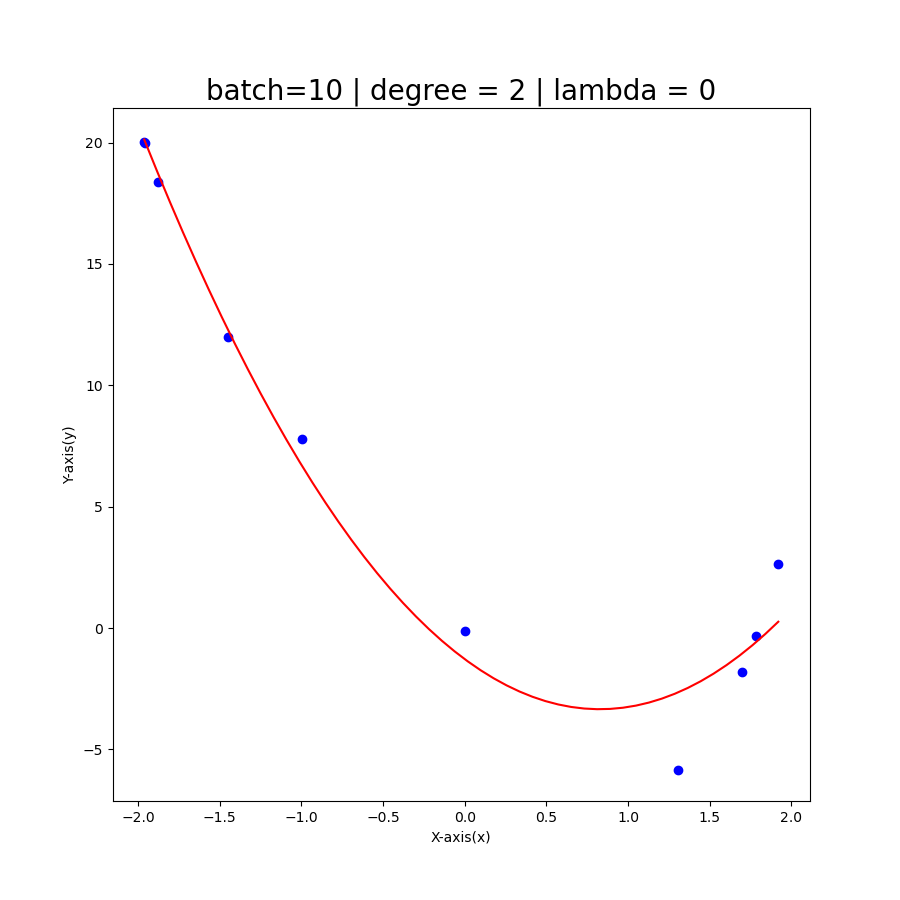
\includegraphics[height=1.5in]{Task 1 Images/Batch 10/Figure_1.png}
    \end{subfigure}%
    ~ 
    \begin{subfigure}[t]{0.25\textwidth}
        \centering
        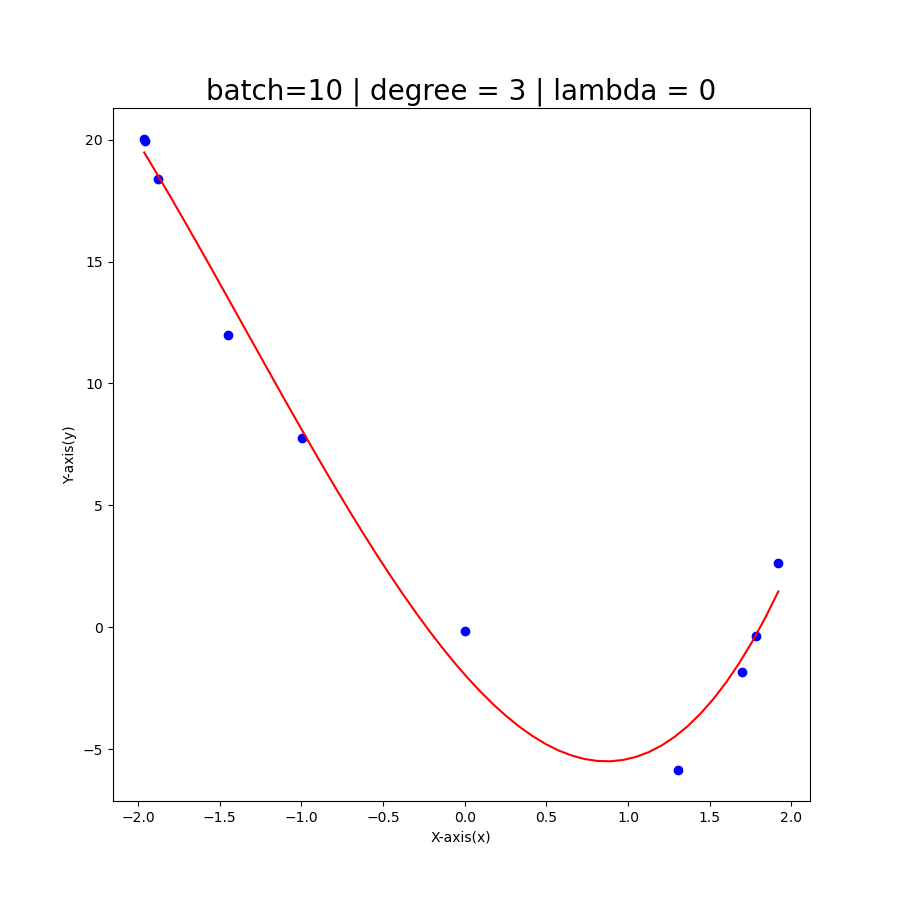
\includegraphics[height=1.5in]{Task 1 Images/Batch 10/Figure_2.png}
    \end{subfigure}%
    ~
    \begin{subfigure}[t]{0.25\textwidth}
        \centering
        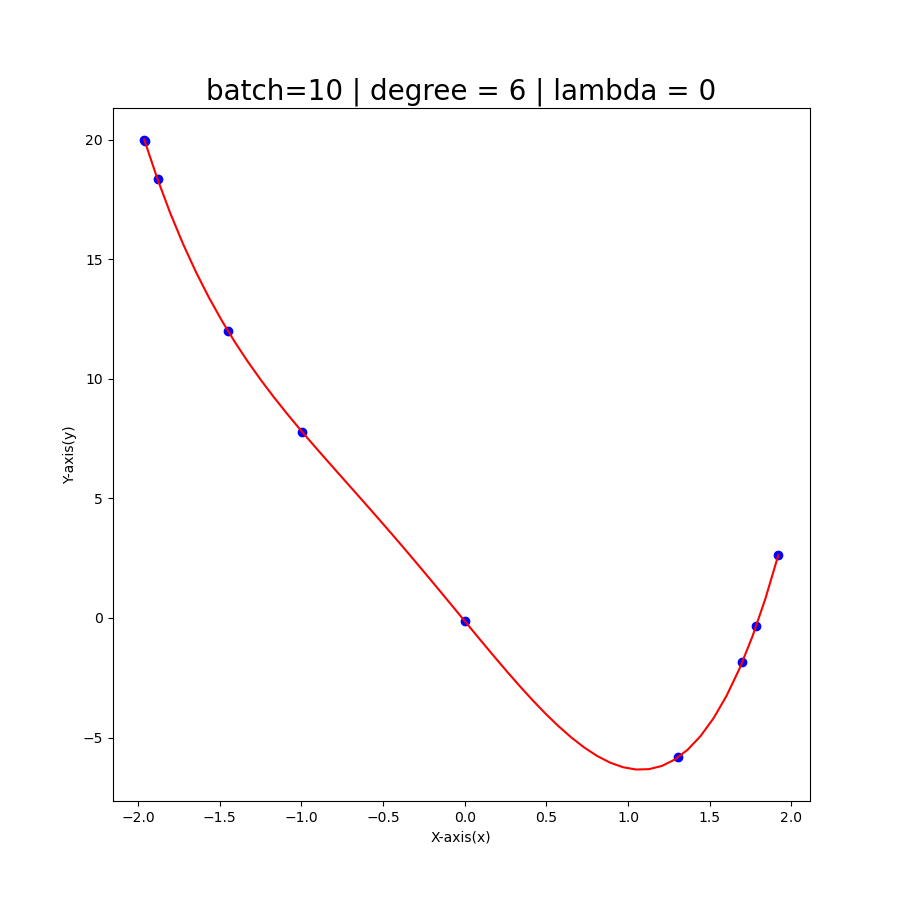
\includegraphics[height=1.5in]{Task 1 Images/Batch 10/Figure_3.png}
    \end{subfigure}%
    ~ 
    \begin{subfigure}[t]{0.25\textwidth}
        \centering
        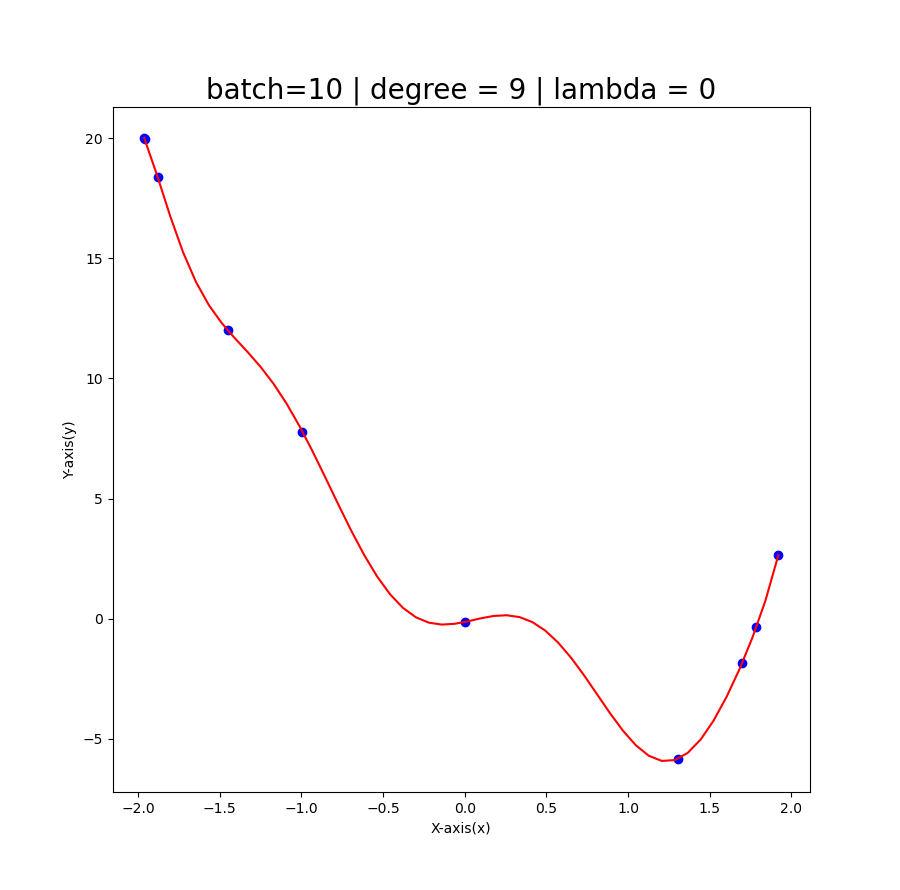
\includegraphics[height=1.5in]{Task 1 Images/Batch 10/Figure_4.png}
    \end{subfigure}%
    \caption{Plots of Polynomials having various orders of degree for a fixed regularisation parameter $\lambda = 0$ using batch size=10}
    \label{fig:1}
\end{figure}


{\rowcolors{3}{green!40!yellow!10}{green!0!yellow!30}
\begin{table}[!ht]
\begin{tabular}{ |p{1.5cm}|p{3cm}|p{3cm}| p{3cm}|  }
\hline
\multicolumn{4}{|c|}{$\mathbf{E}_{rms}$ values for different degrees } \\
\hline
\rowcolor{lightgray} \textbf{Degree} & $\mathbf{E}_{rms-train}$ & $\mathbf{E}_{rms-test}$ & $\mathbf{E}_{rms-valid}$ \\
2   &   1.38  &  1.83   &  2.00   \\   
\hline
 3   &  0.99 &  1.74  &  1.39   \\   
 \hline
 6   &   0.01   &   0.24   &   0.10         \\
 \hline
 9   &   5.4e-4   &    0.19        &     0.42     \\
 \hline
\end{tabular}
\caption{Error comparisons for varying degrees of $\phi(\mathbf{x}) $ for Dataset 1 using batch size=10}
\label{table:1}
\end{table}
}


Since degree 9 is overfit, we experiment with different regularisation parameter lambda the of quadratic regularisation term to see how it affects the fit. For lambda=0.001 and 0.01, the validation Erms decreases than what was before and from 0.1 it increases again. For higher values of lambda the fit is not proper as can be seen from the figures below[\ref{fig:2}].

\newpage
\begin{figure}[!ht]
    \centering
    \begin{subfigure}[ht]{0.5\textwidth}
        \centering
        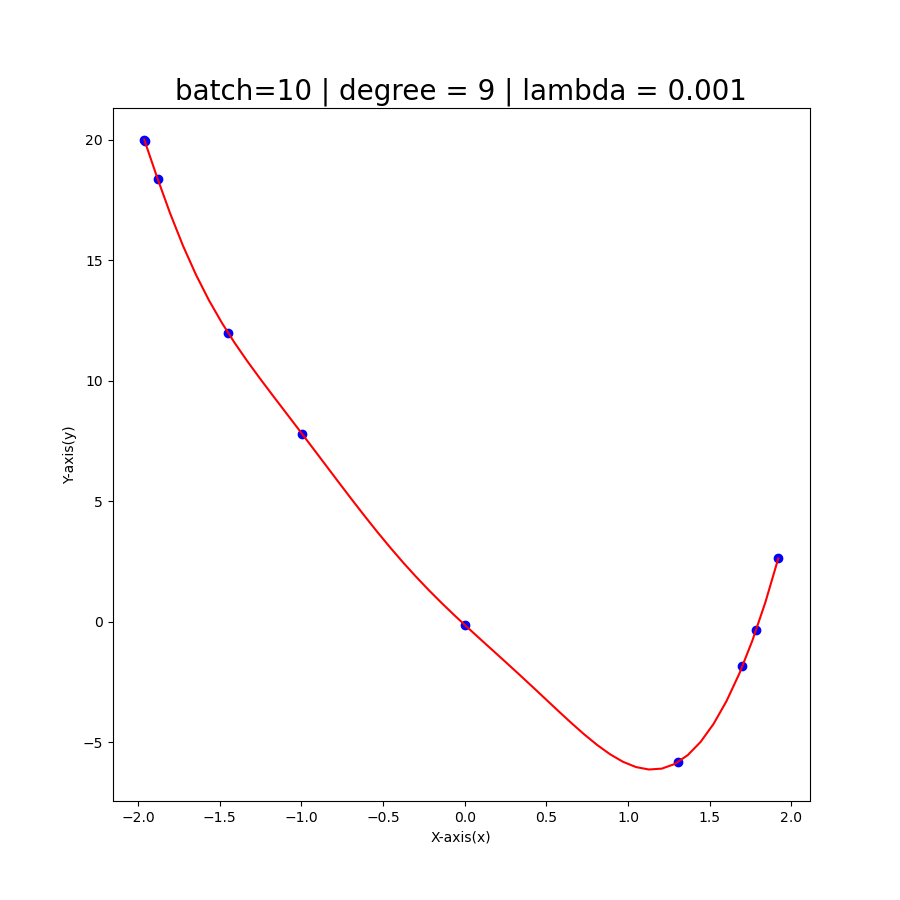
\includegraphics[height=2in]{Task 1 Images/Batch 10/Figure_5.png}
    \end{subfigure}%
    ~ 
    \begin{subfigure}[ht]{0.5\textwidth}
        \centering
        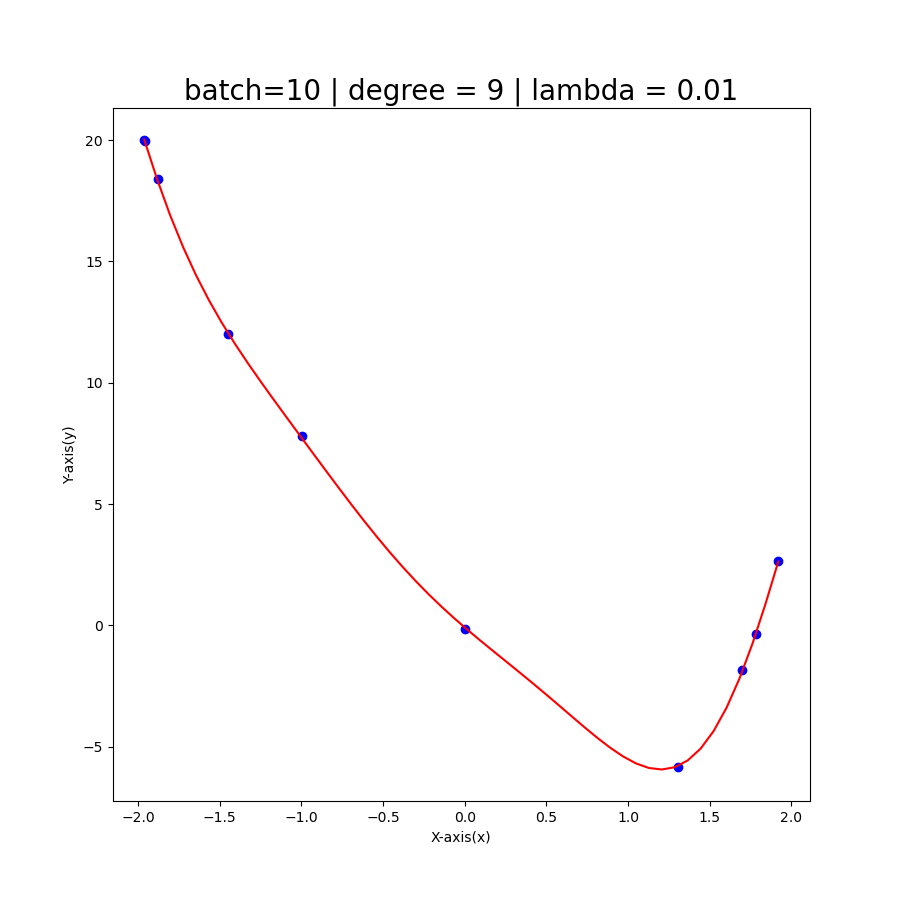
\includegraphics[height=2in]{Task 1 Images/Batch 10/Figure_6.png}
    \end{subfigure}%
    ~
    
    \begin{subfigure}[ht]{0.5\textwidth}
        \centering
        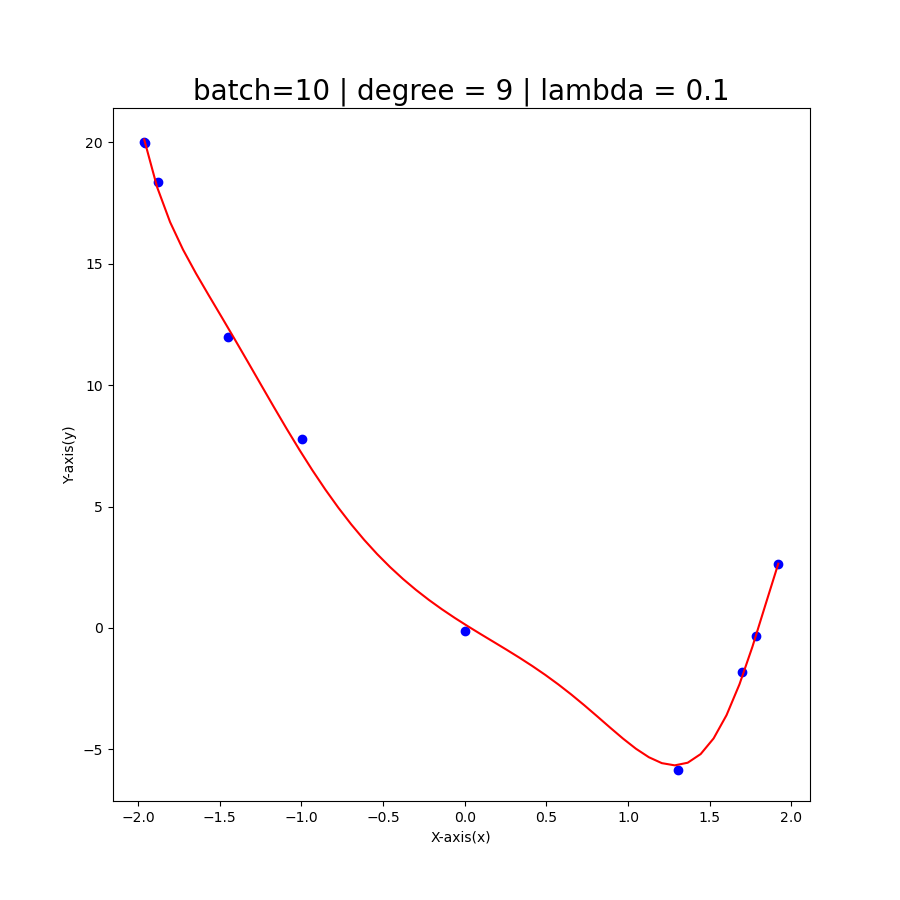
\includegraphics[height=2in]{Task 1 Images/Batch 10/Figure_7.png}
    \end{subfigure}%
    ~ 
    \begin{subfigure}[ht]{0.5\textwidth}
        \centering
        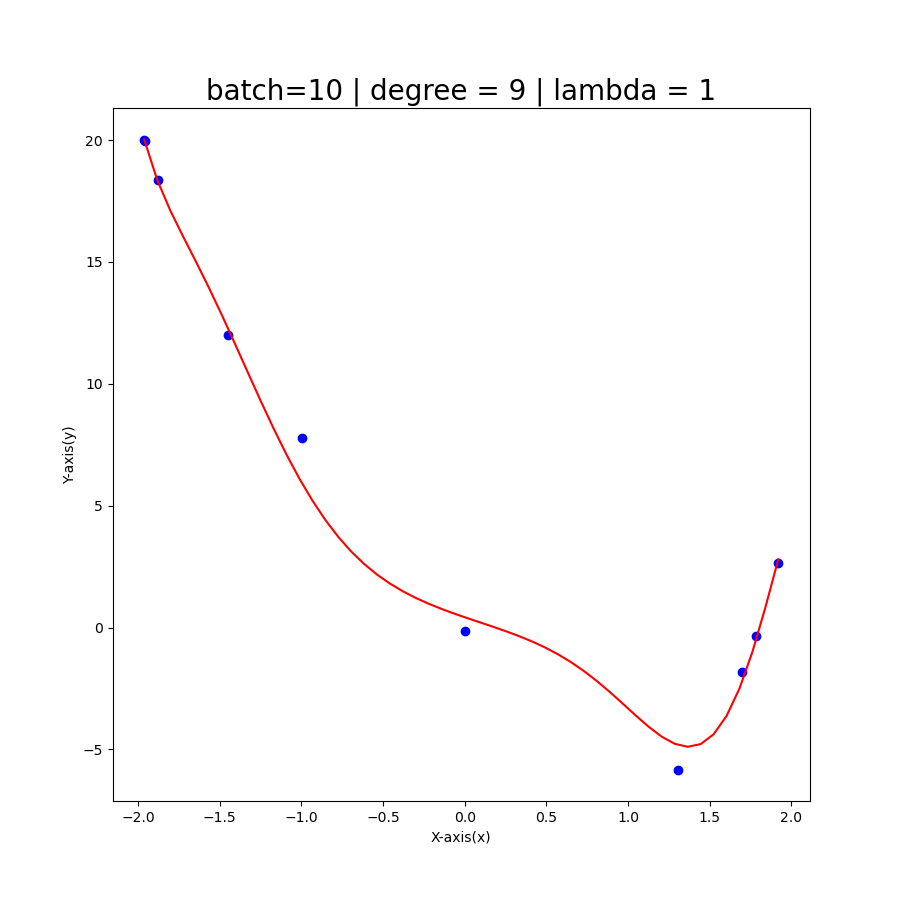
\includegraphics[height=2in]{Task 1 Images/Batch 10/Figure_8.png}
    \end{subfigure}%
    
\end{figure}

\begin{figure}[!ht]
    \centering
    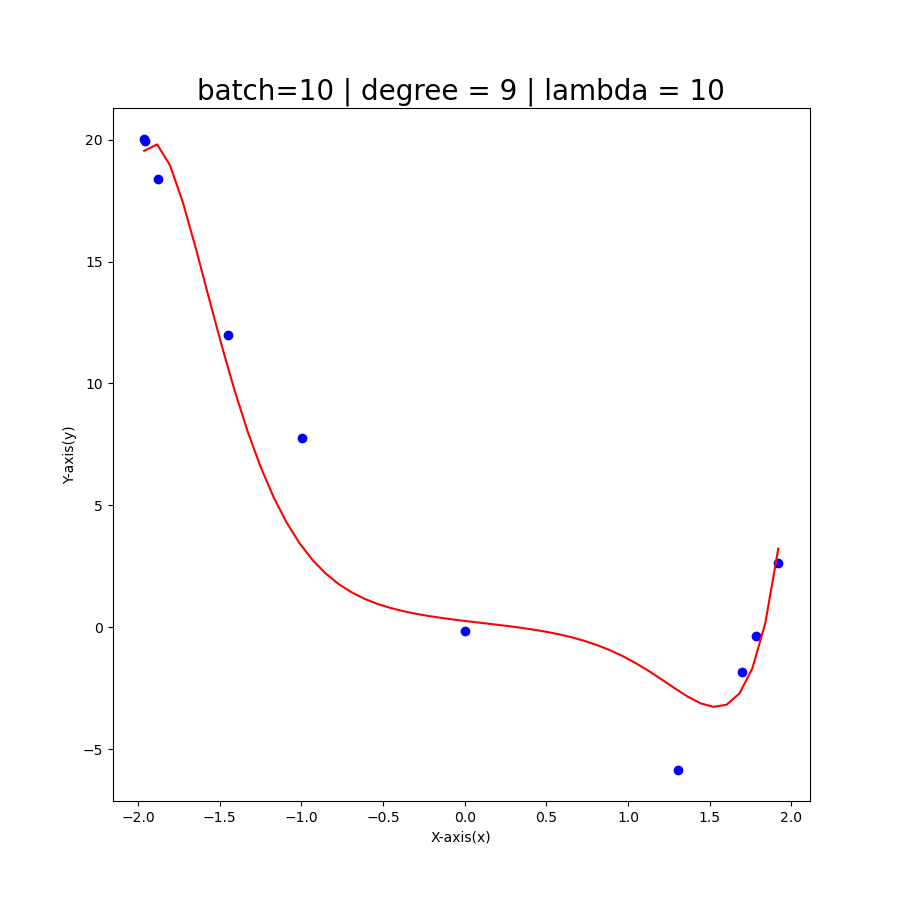
\includegraphics[height=2in]{Task 1 Images/Batch 10/Figure_9.png}
    \caption{Plots of degree 9 Polynomials having various orders of regularisation parameter using batch size=10}
    \label{fig:2}
\end{figure}

{\rowcolors{3}{green!40!yellow!10}{green!0!yellow!30}
\begin{table}[!ht]
\begin{tabular}{ |p{1.5cm}|p{3cm}|p{3cm}| p{3cm}|  }
\hline
\multicolumn{4}{|c|}{$\mathbf{E}_{rms}$ values for different regularisation parameters } \\
\hline
\rowcolor{lightgray} \textbf{lambda} & $\mathbf{E}_{rms-train}$ & $\mathbf{E}_{rms-test}$ & $\mathbf{E}_{rms-valid}$ \\
0.001   &   0.01  &  0.16   &  0.14   \\   
\hline
 0.01   &  0.05 &  0.09  &  0.21   \\   
 \hline
 0.1   &   0.28   &   0.20   &   0.45         \\
 \hline
 1   &   0.71   &    0.41        &     1.15     \\
 \hline
  10   &   1.91   &    0.64        &     2.57     \\
 \hline
\end{tabular}
\caption{Error comparisons for various regularisation parameters with degree=9 for Dataset 1 using batch size=10}
\label{table:2}
\end{table}
}


\subsection{Results for change in regularisation parameter and degree of fit for training data = 200}
Generally at lower degrees, the function does not well fit as can be observed from the plots [\ref{fig:3}]. The fit for degree 6 & 9 seems to be good. Since the validation accuracy is good and the model doesn't seem to overfit, regularisation experiment is not done here.


\begin{figure}[!ht]
    \centering
    \begin{subfigure}[t]{0.25\textwidth}
        \centering
        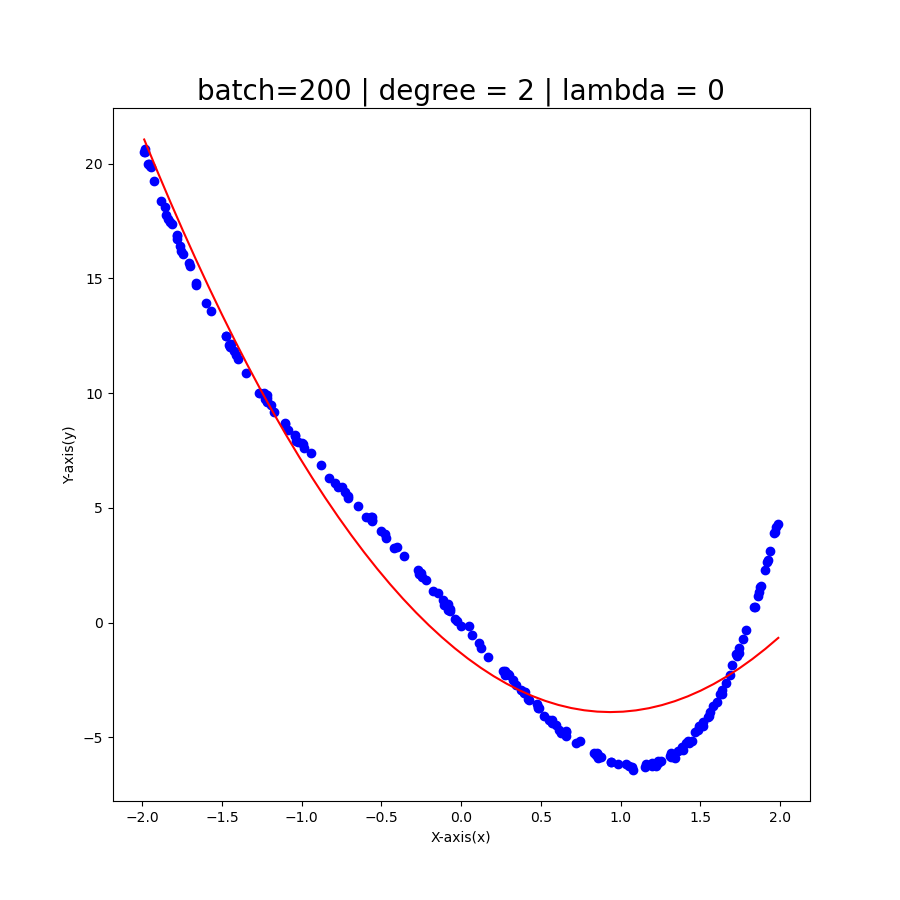
\includegraphics[height=1.5in]{Task 1 Images/Batch 200/Figure_1.png}
    \end{subfigure}%
    ~ 
    \begin{subfigure}[t]{0.25\textwidth}
        \centering
        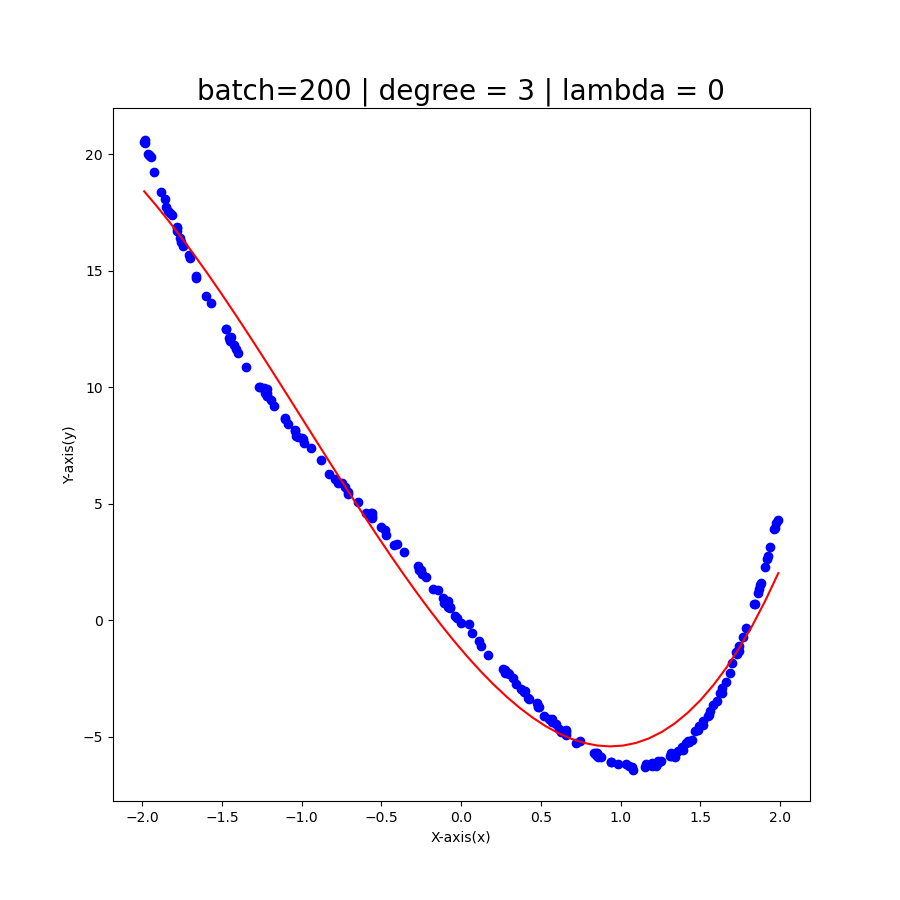
\includegraphics[height=1.5in]{Task 1 Images/Batch 200/Figure_2.png}
    \end{subfigure}%
    ~
    \begin{subfigure}[t]{0.25\textwidth}
        \centering
        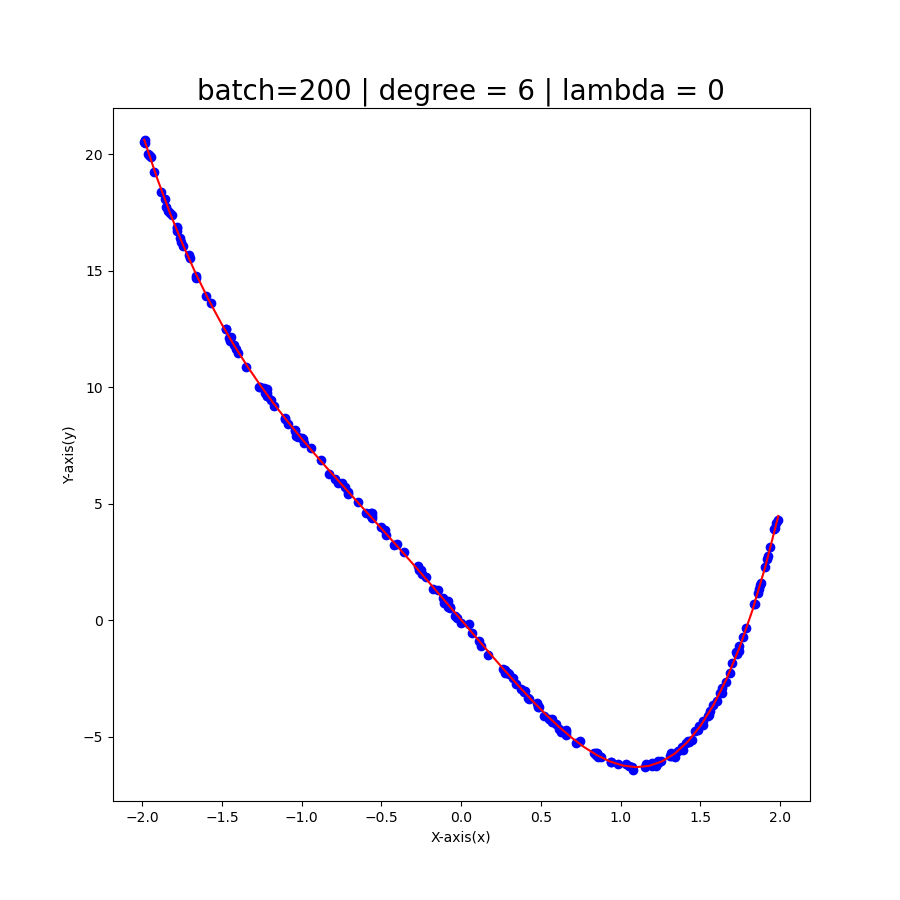
\includegraphics[height=1.5in]{Task 1 Images/Batch 200/Figure_3.png}
    \end{subfigure}%
    ~ 
    \begin{subfigure}[t]{0.25\textwidth}
        \centering
        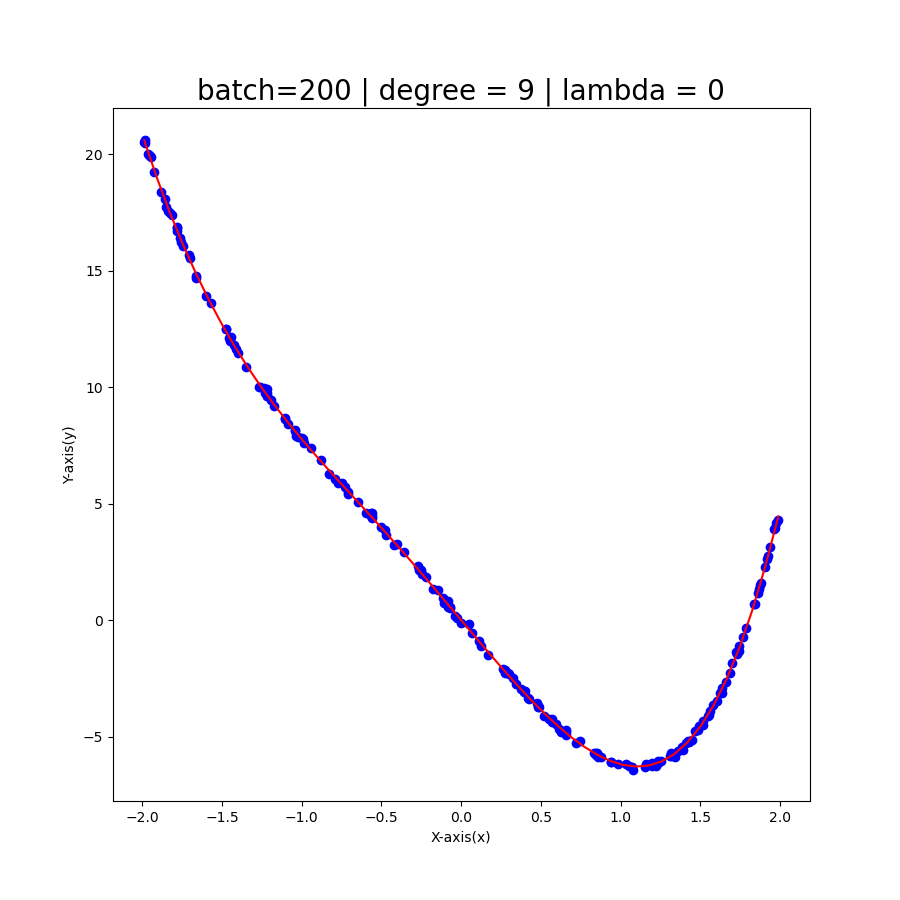
\includegraphics[height=1.5in]{Task 1 Images/Batch 200/Figure_4.png}
    \end{subfigure}%
    \caption{Plots of Polynomials having various orders of degree for a fixed regularisation parameter $\lambda = 0$ using batch size200}
    \label{fig:3}
\end{figure}




{\rowcolors{3}{green!40!yellow!10}{green!0!yellow!30}
\begin{table}[!ht]
\begin{tabular}{ |p{1.5cm}|p{3cm}|p{3cm}| p{3cm}|  }
\hline
\multicolumn{4}{|c|}{$\mathbf{E}_{rms}$ values for different degrees } \\
\hline
\rowcolor{lightgray} \textbf{Degree} & $\mathbf{E}_{rms-train}$ & $\mathbf{E}_{rms-test}$ & $\mathbf{E}_{rms-valid}$ \\
2   &   1.64  &  1.73   &  1.70   \\   
\hline
 3   &  1.05 &  0.85  &  1.07   \\   
 \hline
 6   &   0.09   &   0.09   &   0.11         \\
 \hline
 9   &  0.09   &    0.09        &     0.11     \\
 \hline
\end{tabular}
\caption{Error comparisons for varying degrees of $\phi(\mathbf{x}) $ for Dataset 1 using batch size=200}
\label{table:3}
\end{table}
}
\newpage
\section{Linear Regression for Bivariate Data}

The Polynomial Basis Function used takes the form,

\begin{align*}
    \phi{(\mathbf{x})} &= \{\mathbf{x}_1^i \mathbf{x}_2^j\}
    \intertext{Where, $0 \leq i,j \leq Degree$ and $i+j \leq Degree$ In case of data points with two features, the polynomial basis functions includes,}
    \phi{(\mathbf{x})} &= \{ 1,\mathbf{x}_1, \mathbf{x}_2, \mathbf{x}_1^2, \mathbf{x}_2^2, \mathbf{x}_1\mathbf{x}_2, \mathbf{x}_1^{2}\mathbf{x}_1^{2} \}
\end{align*}


\subsection{Experiments $\And$ Observations on Dataset 2: }

\subsubsection{RMS comparison for varying regularisation parameter $\lambda$ (quadratic regularisation):}

Different $\lambda$ values were tested across different models with the goal of finding any $\lambda$ value that might be able to ameliorate any overfitting. However across all models, the increase of $\lambda$ value was accompanied with the strict increase of RMS value. Therefore, subsequent analysis has been carried out without regularization. The best model which was found to be of $batch = 500$ and $degree = 6$ with no regularisation performed with significant accuracy on the training, test and cross validation without any instances of overfitting. The effect of $\lambda$ is illustrated in the figure[\ref{fig:11}]. The table[\ref{table:3}] illustrates the analysis of different $\lambda$ values across the $degree= 6$ model and it can be inferred without doubt from the table that the best fitting model has $\lambda = 0$.

{\rowcolors{3}{green!40!yellow!10}{green!0!yellow!30}
\begin{table}[!ht]
\centering
\scalebox{0.80}{\begin{tabular}{ |p{1.0cm}|p{3.5cm}|p{3.5cm}| p{3.5cm}|  }
\hline
\multicolumn{4}{|c|}{$\mathbf{E}_{rms}$ values for different data } \\
\hline
\rowcolor{lightgray} \textbf{$\lambda$} & $\mathbf{E}_{rms-train}$ & $\mathbf{E}_{rms-test}$ & $\mathbf{E}_{rms-valid}$ \\
\hline
 1   &   7.58e-06  &  1.06e-05   &  7.51e-06   \\   
 \hline
 0   &   1.21e-07   &   1.15e-07  &   1.17e-07         \\
 \hline
 0.1   &   7.75e-06   &    1.06e-06     &     7.77e-07     \\
 \hline
 0.01  &   1.04e-07    &    1.31e-07   &     1.01e-07    \\
 \hline
 0.001  &   1.18e-07  &    1.08-07       &     1.17e-07      \\
 \hline
 0.0001  &   3.30e-08     &     3.2e-08      &      3.08e-08   \\
 \hline
 1e-05   &   1.77e-07    &     1.65e-07      &     1.69e-07  \\
\hline
\end{tabular}}
\caption{Error comparisons for varying values of $\lambda $ for Dataset 2 and a model of $degree = 6$}.
\label{table:4}
\end{table}
}


\begin{figure}[!ht]
    \centering
    \begin{subfigure}[t]{0.25\textwidth}
        \centering
        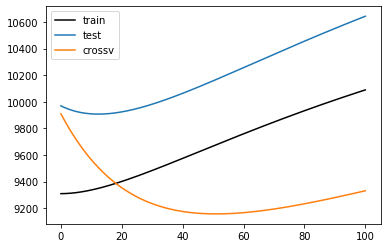
\includegraphics[height=1in]{Task 2 Images/batch500_deg2_lambda.png}
        \caption{Degree, $M = 2$}
    \end{subfigure}%
    ~ 
    \begin{subfigure}[t]{0.25\textwidth}
        \centering
        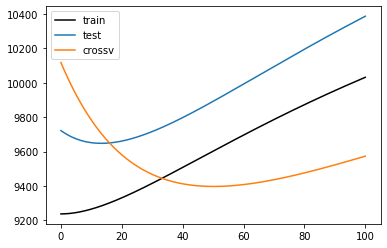
\includegraphics[height=1in]{Task 2 Images/batch500_deg3_lambda.png}
        \caption{Degree, $M = 3$ }
    \end{subfigure}%
    ~
    \begin{subfigure}[t]{0.25\textwidth}
        \centering
        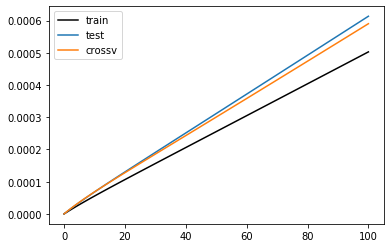
\includegraphics[height=1in]{Task 2 Images/batch500_deg6_lambda1to100.png}
        \caption{ Degree, $M = 6$}
    \end{subfigure}
    \caption{Effect of $\lambda$}
    \label{fig:11}
\end{figure}





\subsubsection{RMS comparison across different models}

Tables [\ref{table:5}], [\ref{table:6}], [\ref{table:7}], and [\ref{table:8}] provides an error based analysis of the model implemented.

{\rowcolors{3}{green!40!yellow!10}{green!0!yellow!30}
\begin{table}[!h]
\begin{tabular}{ |p{1.5cm}|p{3cm}|p{3cm}| p{3cm}|  }
\hline
\multicolumn{4}{|c|}{$\mathbf{E}_{rms}$ values for different data } \\
\hline
\rowcolor{lightgray} Degree & $\mathbf{E}_{rms-train}$ & $\mathbf{E}_{rms-test}$ & $\mathbf{E}_{rms-valid}$ \\
\hline
 2   &   8472.09  &  7916.24  &  11603.31   \\   
 \hline
 3   &   7746.87   &   10209.22  &   9055.03   \\
 \hline
 6   &   1.11e-06   &    7.12e-06     &     1.032e-06    \\
\hline
\end{tabular}
\caption{Error comparisons for varying degrees $\phi(\mathbf{x}) $ for Dataset 2 using 50 samples}.
\label{table:5}
\end{table}

\begin{table}[!h]
 \vspace*{\floatsep}
 \begin{tabular}{ |p{1.5cm}|p{3cm}|p{3cm}| p{3cm}|  }
\hline
\multicolumn{4}{|c|}{$\mathbf{E}_{rms}$ values for different data } \\
\hline
\rowcolor{lightgray} Degree & $\mathbf{E}_{rms-train}$ & $\mathbf{E}_{rms-test}$ & $\mathbf{E}_{rms-valid}$ \\
\hline
 2   &   7836.93  &  9102.67 &  10203.59  \\   
 \hline
 3   &   7410.93  &   8955.31 &   9615.30    \\
 \hline
 6   &   9.07e-08   &    1.14e-07     &     9.06e-08    \\
\hline
\end{tabular}
\caption{Error comparisons for varying degrees $\phi(\mathbf{x}) $ for Dataset 2 using 100 samples}.
\label{table:6}
\end{table}

\begin{table}[!h]
\vspace*{\floatsep}
 \begin{tabular}{ |p{1.5cm}|p{3cm}|p{3cm}| p{3cm}|  }
\hline
\multicolumn{4}{|c|}{$\mathbf{E}_{rms}$ values for different data } \\
\hline
\rowcolor{lightgray} Degree & $\mathbf{E}_{rms-train}$ & $\mathbf{E}_{rms-test}$ & $\mathbf{E}_{rms-valid}$ \\
\hline
 2   &   9007.85  &  9941.50 & 7712.90   \\   
 \hline
 3   &   8891.04   &   10448.97  &   7669.04    \\
 \hline
 6   &   2.77e-08   &    3.15e-08     &     3.17e-08   \\
\hline
\end{tabular}
\caption{Error comparisons for varying degrees $\phi(\mathbf{x}) $ for Dataset 2 using 200 samples}.
\label{table:7}
\end{table}

\begin{table}[!ht]
\vspace*{\floatsep}
 \begin{tabular}{ |p{1.5cm}|p{3cm}|p{3cm}| p{3cm}|  }
\hline
\multicolumn{4}{|c|}{$\mathbf{E}_{rms}$ values for different data } \\
\hline
\rowcolor{lightgray} Degree & $\mathbf{E}_{rms-train}$ & $\mathbf{E}_{rms-test}$ & $\mathbf{E}_{rms-valid}$ \\
\hline
 2   &   9308.74  &  9968.55 & 9908.81   \\   
 \hline
 3   &   9237.93   &   9721.98  &   10117.44    \\
 \hline
 6   &   2.54e-08   &    2.92e-08     &     2.51e-08  \\
\hline
\end{tabular}
\caption{Error comparisons for varying degrees $\phi(\mathbf{x}) $ for Dataset 2 using 500 samples}.
\label{table:8}
\end{table}
}


\newpage
\subsubsection{Surface Plots with Training set superimposed}
Figures [\ref{fig:12}], [\ref{fig:13}], [\ref{fig:14}] and [\ref{fig:15}] are the various surface plots.

\begin{figure}[!ht]
    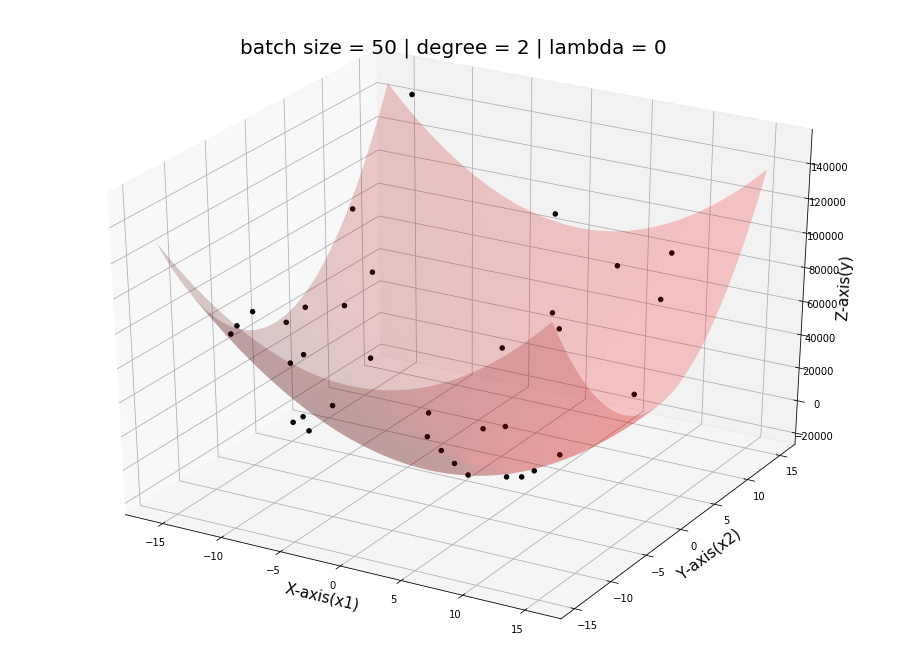
\includegraphics[width=.30\textwidth]{Task 2 Images/surfaceplot_batch50_deg2_lamb0.png}\hfill
    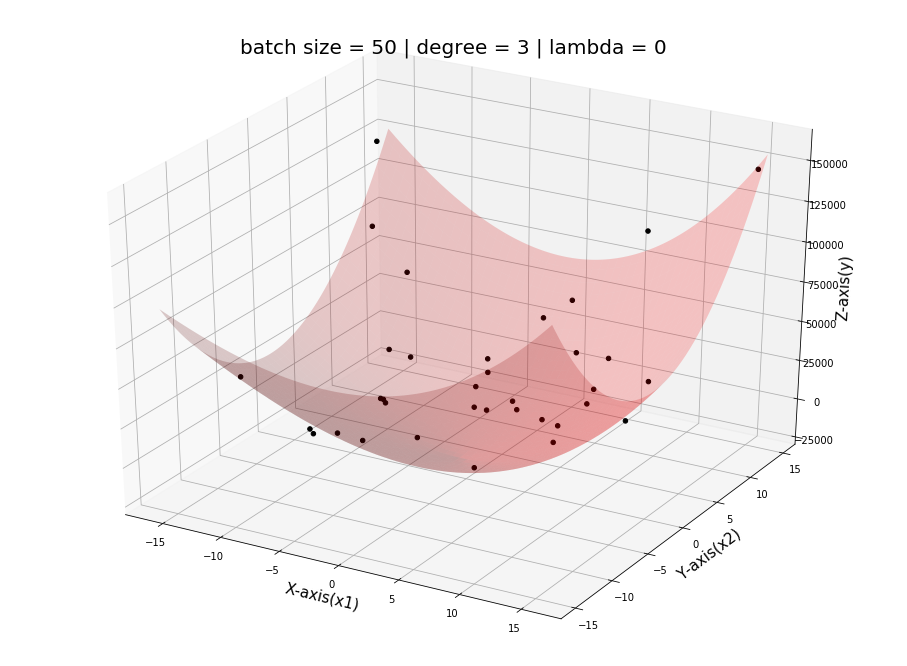
\includegraphics[width=.30\textwidth]{Task 2 Images/surfaceplot_batch50_deg3_lamb0.png}\hfill
    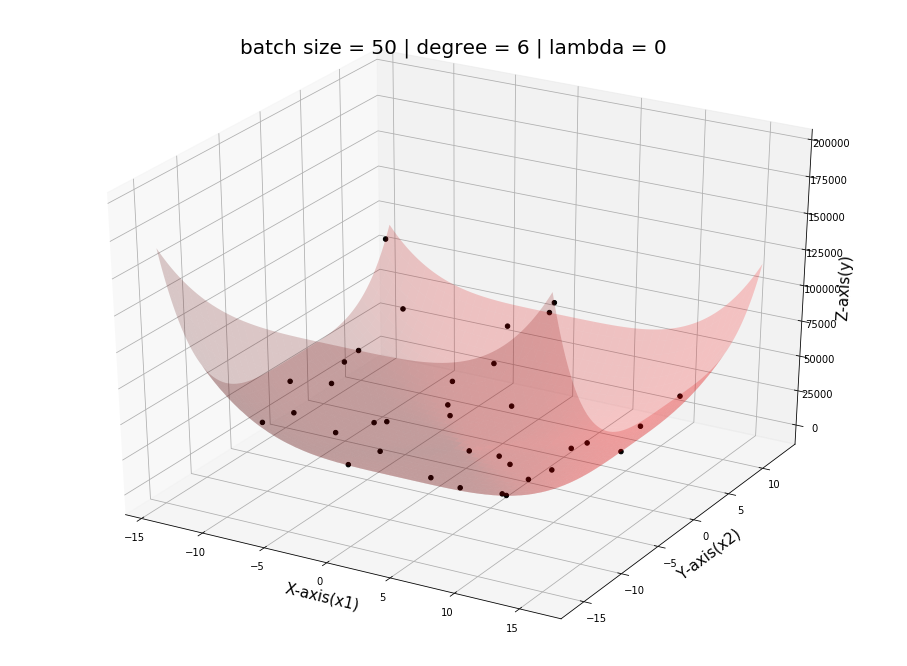
\includegraphics[width=.30\textwidth]{Task 2 Images/surfaceplot_batch50_deg6_lamb0.png}
    \caption{Surface Plots using various degree for a fixed best regularisation parameter $\lambda = 0$ using 50 samples }
    \label{fig:12}
\end{figure}

\begin{figure}[!ht]
    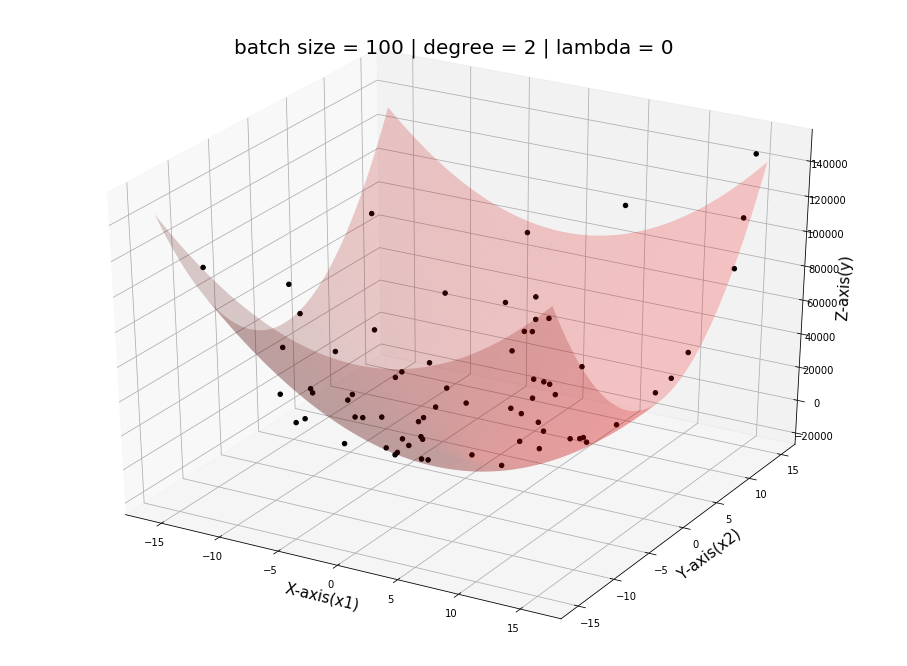
\includegraphics[width=.30\textwidth]{Task 2 Images/surfaceplot_batch100_deg2_lamb0.png}\hfill
    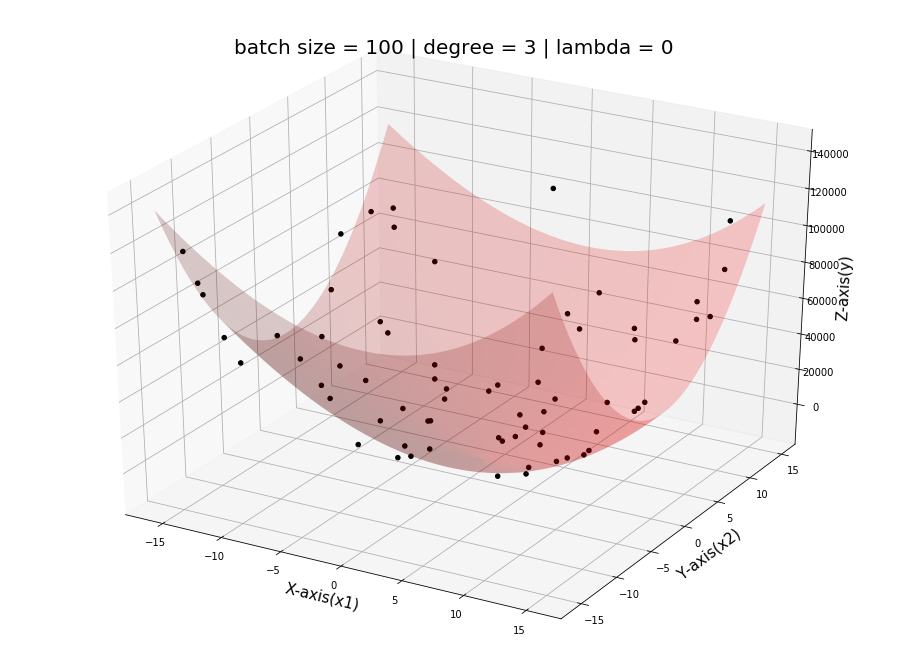
\includegraphics[width=.30\textwidth]{Task 2 Images/surfaceplot_batch100_deg3_lamb0.png}\hfill
    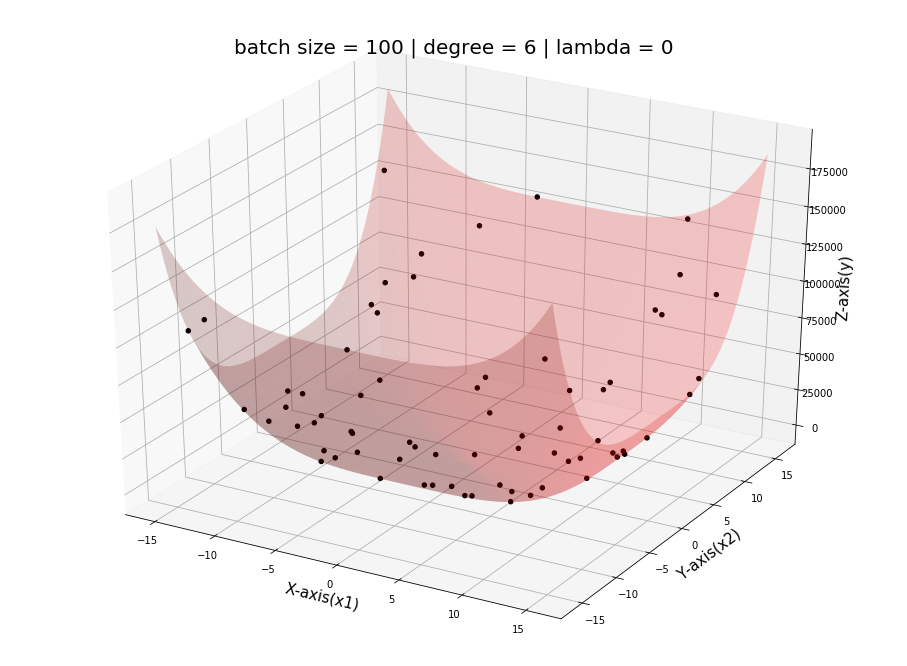
\includegraphics[width=.30\textwidth]{Task 2 Images/surfaceplot_batch100_deg6_lamb0.png}
    \caption{Surface Plots using various degree for a fixed regularisation parameter $\lambda = 0$ using 100 samples}
    \label{fig:13}
\end{figure}

\begin{figure}[!ht]
    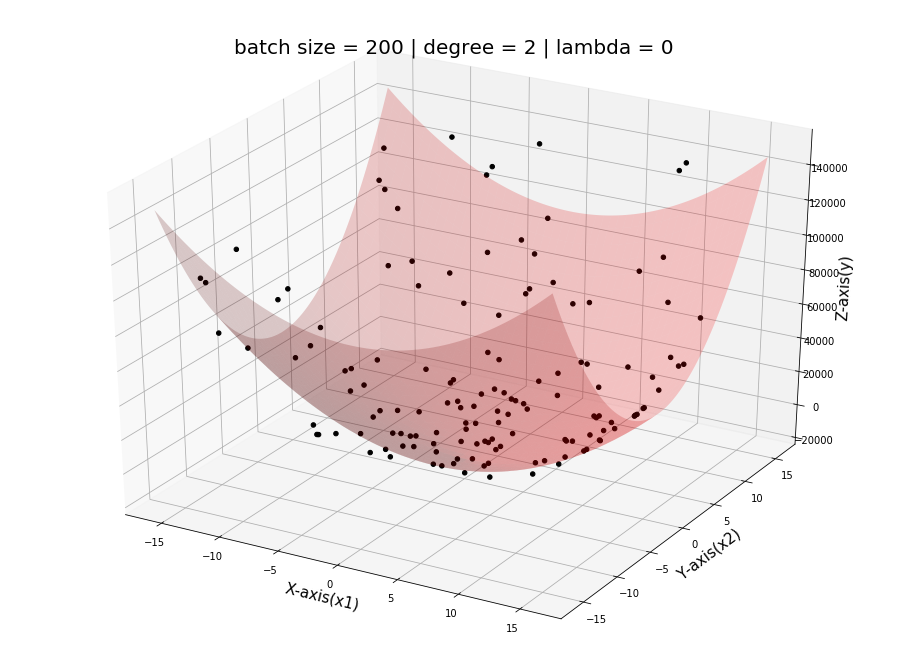
\includegraphics[width=.30\textwidth]{Task 2 Images/surfaceplot_batch200_deg2_lamb0.png}\hfill
    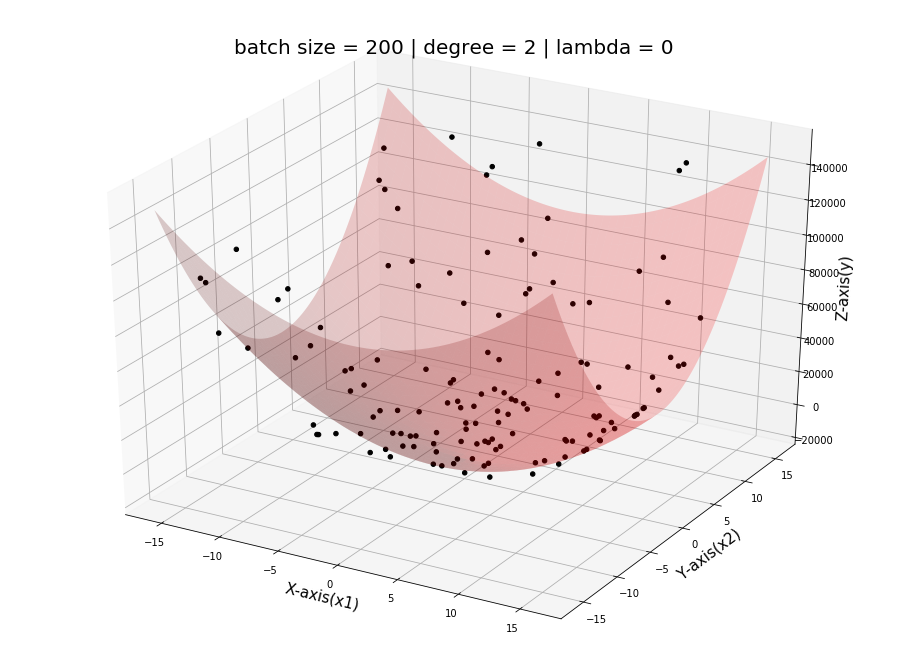
\includegraphics[width=.30\textwidth]{Task 2 Images/surfaceplot_batch200_deg2_lamb0.png}\hfill
    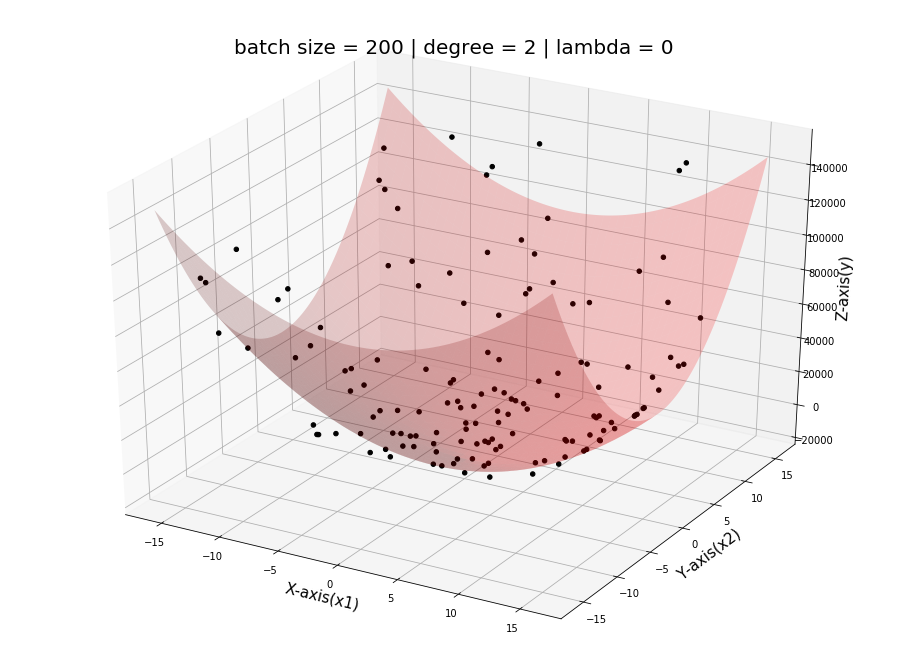
\includegraphics[width=.30\textwidth]{Task 2 Images/surfaceplot_batch200_deg2_lamb0.png}
    \caption{Surface Plots using various degree for a fixed regularisation parameter $\lambda = 0$ using 200 samples}
    \label{fig:14}
 \end{figure}


\begin{figure}[!ht] 
    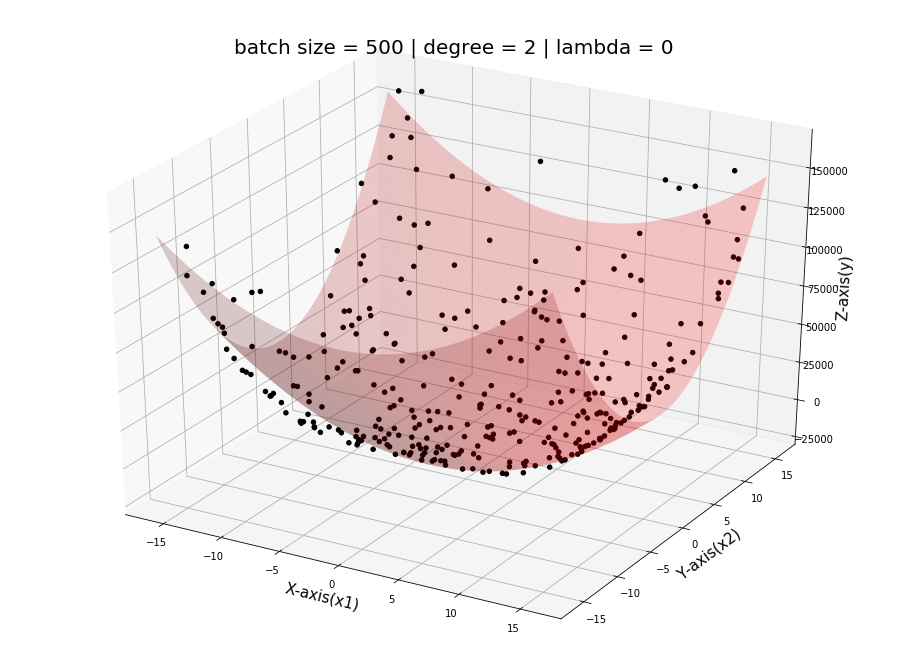
\includegraphics[width=.30\textwidth]{Task 2 Images/surfaceplot_batch500_deg2_lamb0.png}\hfill
    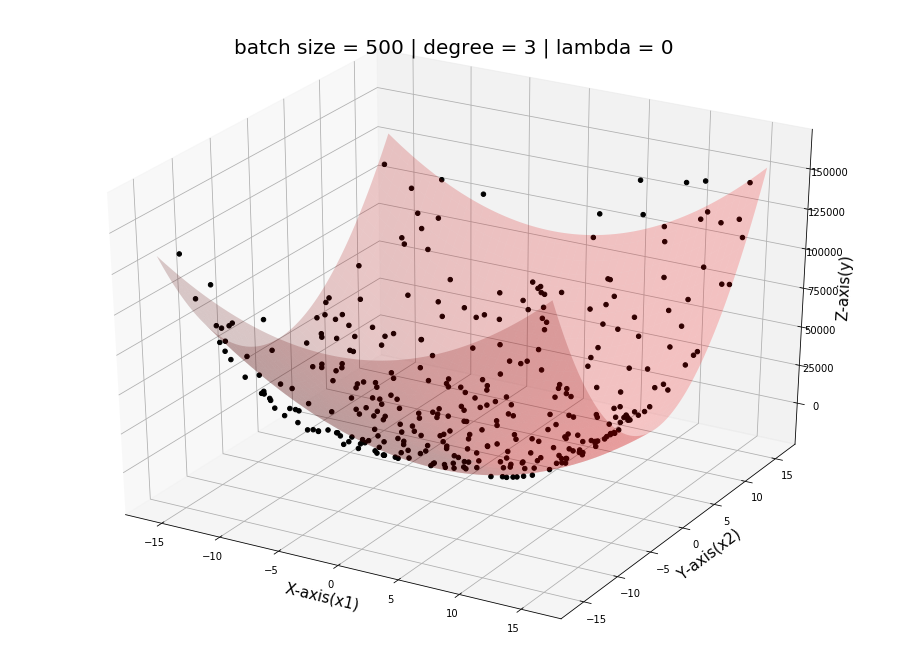
\includegraphics[width=.30\textwidth]{Task 2 Images/surfaceplot_batch500_deg3_lamb0.png}\hfill
    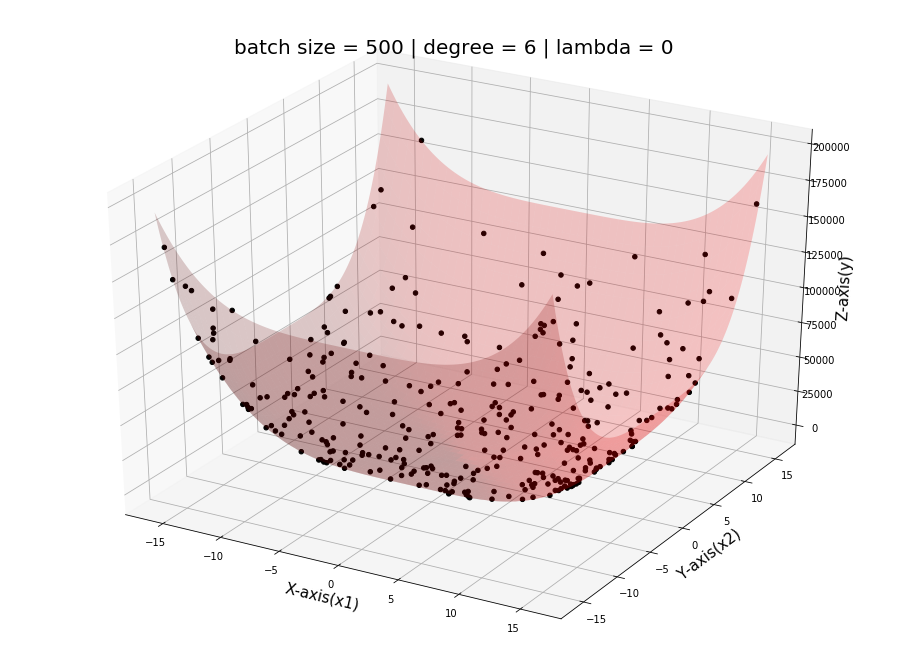
\includegraphics[width=.30\textwidth]{Task 2 Images/surfaceplot_batch500_deg6_lamb0.png}
    \caption{Surface Plots using various degree for a fixed regularisation parameter $\lambda = 0$ using 500 samples}
    \label{fig:15}
\end{figure}

\newpage
\subsubsection{Scatter Plots of the Best Model}
The best model was found to be of batch size 500 and degree 6 without any regularization and fared significantly better than the other degree 2,3 models as it's $E_{rms}$ values were found to be smaller in orders of magnitude $10^9$. Scatter plots of the best model are represented in figure [\ref{fig:16}]


 \begin{figure}[!ht]
     \centering
     \begin{subfigure}[t]{0.30\textwidth}
         \centering
         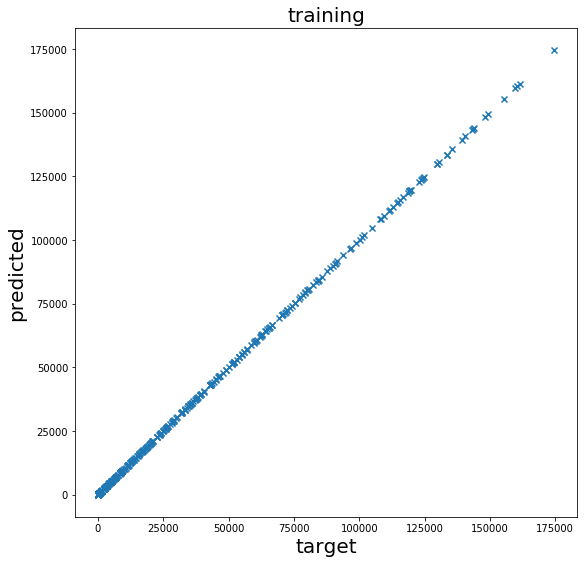
\includegraphics[height=1.6in]{Task 2 Images/best_scatterplot_batch_500_degree_6_lambda_0_training.png}
         \caption{Training Data}
     \end{subfigure}%
     ~ 
     \begin{subfigure}[t]{0.30\textwidth}
         \centering
         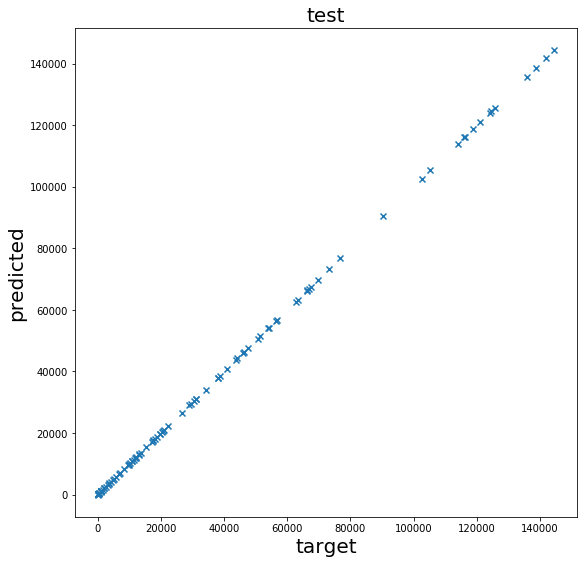
\includegraphics[height=1.6in]{Task 2 Images/best_scatterplot_batch_500_degree_6_lambda_0_test.png}
         \caption{Test Data }
     \end{subfigure}%
     ~
     \begin{subfigure}[t]{0.30\textwidth}
         \centering
         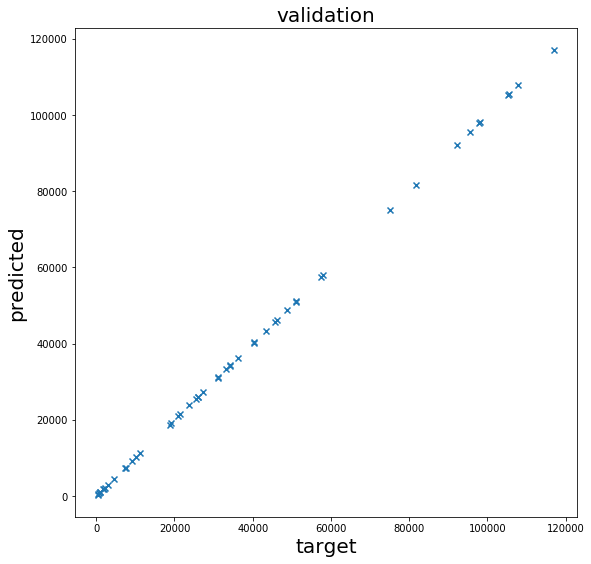
\includegraphics[height=1.6in]{Task 2 Images/best_scatterplot_batch_500_degree_6_lambda_0_validation.png}
         \caption{Validation Data }
     \end{subfigure}
     \caption{Best Scatter Plot}
     \label{fig:16}
\end{figure}

\newpage
\section{Linear Regression for Multivariate Real World Data  $\And$ Bivariate Data}
The model implemented here makes use of a Gaussian Basis Function,
\begin{equation*}
    \mathbb{\phi}_j(\mathbf{x}) = \exp \left( {-\frac{(\mathbf{x} - \mu_j)^2}{\sigma^2}} \right)
\end{equation*}

\subsection{Experiments $\And$ Observations on Dataset 2:}

\subsubsection{RMS error comparison for varying dimensions and width of $\mathbb{\phi}(\mathbf{x})$:}

A total of 500 samples from the given bivariate dataset was chosen at random and divided in to training, validation and test data(70$\%$, 20$\%$ and 10$\%$). Using the training data thus generated an attempt is made to find the best model. At first the case without regularisation is considered. For each dimension of the gaussian basis function, different values of width has been experimented here. As can be concluded from the tables, a dimension of 75 and width of 10 seems to be optimal model for the regression task at hand. Also, one can observe over-fitting when the dimensions are increased to 340 and for width of 1. The value of training data, $E_{rms}$ is drastically lower than that of validation data.

{\rowcolors{3}{green!40!yellow!10}{green!0!yellow!30}
\begin{table}[hptb]
\begin{tabular}{ |p{1.5cm}|p{3cm}|p{3cm}| p{3cm}|  }
\hline
\multicolumn{4}{|c|}{$\mathbf{E}_{rms}$ values for dimension $25$ } \\
\hline
\rowcolor{lightgray} \textbf{Width} & $\mathbf{E}_{rms-train}$ & $\mathbf{E}_{rms-val}$ & $\mathbf{E}_{rms-test}$ \\
\hline
  1   &   $3.40 \times 10^4$   &  $6.42 \times 10^4 $        &     $4.16 \times 10^4 $   \\
 \hline
 10   &   $3.07 \times 10^3$  &  $4.12 \times 10^3 $          &     $3.17 \times 10^3 $   \\
 \hline
 50   &   $1.96 \times 10^5$  & $2.01 \times 10^5$          &         $2.08 \times 10^5$   \\
\hline
\end{tabular}
\label{table:8}
\end{table}
}
{\rowcolors{3}{green!40!yellow!10}{green!0!yellow!30}
\begin{table}[hptb]
\begin{tabular}{ |p{1.5cm}|p{3cm}|p{3cm}| p{3cm}|  }
\hline
\multicolumn{4}{|c|}{$\mathbf{E}_{rms}$ values for dimension $50$ } \\
\hline
\rowcolor{lightgray} \textbf{Width} & $\mathbf{E}_{rms-train}$ & $\mathbf{E}_{rms-val}$ & $\mathbf{E}_{rms-test}$ \\
\hline
  1   &   $2.70 \times 10^4$   &  $4.39 \times 10^4 $        &     $5.50 \times 10^4 $   \\
 \hline
 10   &   $3.33 \times 10^2$  &  $4.87 \times 10^2 $          &     $4.46 \times 10^2 $   \\
 \hline
 50   &   $7.01 \times 10^5$  & $6.86 \times 10^5$          &         $6.72 \times 10^5$   \\
\hline
\end{tabular}
\label{table:8}
\end{table}
}
{\rowcolors{3}{green!40!yellow!10}{green!0!yellow!30}
\begin{table}[hptb]
\begin{tabular}{ |p{1.5cm}|p{3cm}|p{3cm}| p{3cm}|  }
\hline
\multicolumn{4}{|c|}{$\mathbf{E}_{rms}$ values for dimension $75$ } \\
\hline
\rowcolor{lightgray} \textbf{Width} & $\mathbf{E}_{rms-train}$ & $\mathbf{E}_{rms-val}$ & $\mathbf{E}_{rms-test}$ \\
\hline
  1   &   $2.28 \times 10^4$   &  $3.56 \times 10^4 $        &     $4.79 \times 10^4 $   \\
 \hline
 10   &   $1.18 \times 10^2$  &  $1.47 \times 10^2 $          &     $1.34 \times 10^2 $   \\
 \hline
 50   &   $3.84 \times 10^5$  & $3.94 \times 10^5$          &         $4.05 \times 10^5$   \\
\hline
\end{tabular}
\label{table:8}
\end{table}
}
{\rowcolors{3}{green!40!yellow!10}{green!0!yellow!30}
\begin{table}[hptb]
\begin{tabular}{ |p{1.5cm}|p{3cm}|p{3cm}| p{3cm}|  }
\hline
\multicolumn{4}{|c|}{$\mathbf{E}_{rms}$ values for dimension $340$ } \\
\hline
\rowcolor{lightgray} \textbf{Width} & $\mathbf{E}_{rms-train}$ & $\mathbf{E}_{rms-val}$ & $\mathbf{E}_{rms-test}$ \\
\hline
  1   &   $1.01 \times 10^3$   &  $2.51 \times 10^4 $        &     $1.97 \times 10^4 $   \\
 \hline
 10   &   $2.74 \times 10^6$  &  $3.30 \times 10^6 $          &     $3.41 \times 10^6 $   \\
 \hline
 50   &   $5.22 \times 10^5$  & $5.29 \times 10^5$          &         $5.32 \times 10^5$   \\
\hline
\end{tabular}
\caption{Error comparisons for varying values of $\phi(\mathbf{x}) $  and width($\sigma$) for Dataset 2}
\label{table:8}
\end{table}
}

\newpage
\subsubsection{Effect of regularisation in case of over-fitting:}

As inferred from the previous section, the over-fit case of dimension 340 and width 1 is experimented for different values of $\lambda$, thus a regularisation term is added resulting in various models for fixed dimension and width. Both quadratic and tikhonov regulariser are experimented with here. This helps us to see the impact of regularisation in case of over-fitting. As can be seen from the error values, though adding a regulariser doesn't better fit the model but it helps in ruling out models which have essentially memorized the training data-set but perform poorily on test data set.

{\rowcolors{3}{green!40!yellow!10}{green!0!yellow!30}
\begin{table}[hptb]
\begin{tabular}{ |p{1.5cm}|p{3cm}|p{3cm}| p{3cm}|  }
\hline
\multicolumn{4}{|c|}{$\mathbf{E}_{rms}$ values for different data } \\
\hline
\rowcolor{lightgray} $\lambda$ & $\mathbf{E}_{rms-train}$ & $\mathbf{E}_{rms-val}$ & $\mathbf{E}_{rms-test}$ \\
\hline
  10e-5  &  $1.07 \times 10^3$       &       $2.517 \times 10^4$ & $1.979 \times 10^4$  \\
 \hline
  10e-3  &   $1.08 \times 10^3$       &       $2.520 \times 10^4$        &     $1.974 \times 10^4$     \\
 \hline
  10e-1  &   $1.17 \times 10^3$       &       $2.529 \times 10^4$       &     $1.983 \times 10^4$    \\
 \hline
  0  &    $1.01 \times 10^3$     &      $2.516 \times 10^4 $         &     $1.979 \times 10^4$      \\
  \hline
  10     &   $2.84 \times 10^4$   &        $3.852 \times 10^4$         &     $3.782 \times 10^4$      \\
  \hline
  10e+03   &   $5.11 \times 10^4$    &         $5.919 \times 10^4$      &      $6.081 \times 10^4$        \\
  \hline
  10e+05  &    $5.20 \times 10^4$  &         $6.001 \times 10^4$       &        $6.170 \times 10^4$      \\
\hline
\end{tabular}
\caption{Error comparisons for quadratic regularisation by varying $\lambda $  and fixed dimension =340 and width = 1 for Dataset 2}
\label{table:9}
\end{table}
}


{\rowcolors{3}{green!40!yellow!10}{green!0!yellow!30}
\begin{table}[hptb]
\begin{tabular}{ |p{1.5cm}|p{3cm}|p{3cm}| p{3cm}|  }
\hline
\multicolumn{4}{|c|}{$\mathbf{E}_{rms}$ values for different data } \\
\hline
\rowcolor{lightgray} $\lambda$ & $\mathbf{E}_{rms-train}$ & $\mathbf{E}_{rms-val}$ & $\mathbf{E}_{rms-test}$ \\
\hline
  10e-3  &   $1.007 \times 10^3$       &       $2.543 \times 10^4$        &     $1.970 \times 10^4$     \\
 \hline
  10e-1  &   $1.046 \times 10^3$       &       $3.088 \times 10^4$       &     $2.763 \times 10^4$    \\
 \hline
  0  &    $1.007 \times 10^3$     &      $2.516 \times 10^4 $         &     $1.979 \times 10^4$      \\
  \hline
  10     &   $3.161 \times 10^4$   &        $4.01 \times 10^4$         &     $3.930 \times 10^4$      \\
  \hline
  10e+03   &   $5.119 \times 10^4$    &         $5.920 \times 10^4$      &      $6.080 \times 10^4$        \\
  \hline
  10e+05  &    $5.204 \times 10^4$  &         $6.005 \times 10^4$       &        $6.170 \times 10^4$      \\
\hline
\end{tabular}
\caption{Error comparisons for tikhonov regularisation by varying $\lambda $  and fixed dimension =340 and width = 1 for Dataset 2}
\label{table:10}
\end{table}
}

\newpage
\subsubsection{Scatter Plots of Best Model}
Figure [\ref{fig:17}] shows the the scatter plot of predicted and actual target variable for the training and the test data.

\begin{figure}[h]
    \centering
    \begin{subfigure}[t]{0.50\textwidth}
        \centering
        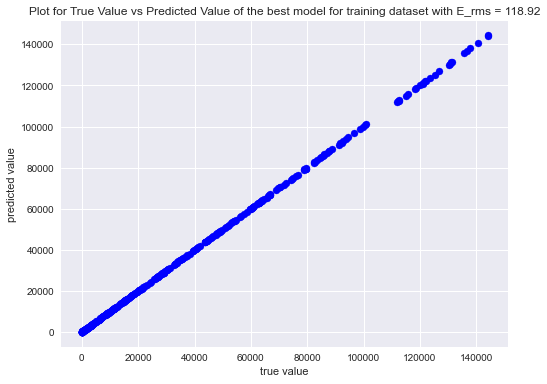
\includegraphics[height=1.6in]{Task3_new_images/batch500_tr.png}
        \caption{Training Data}
    \end{subfigure}%
    ~ 
    \begin{subfigure}[t]{0.50\textwidth}
        \centering
        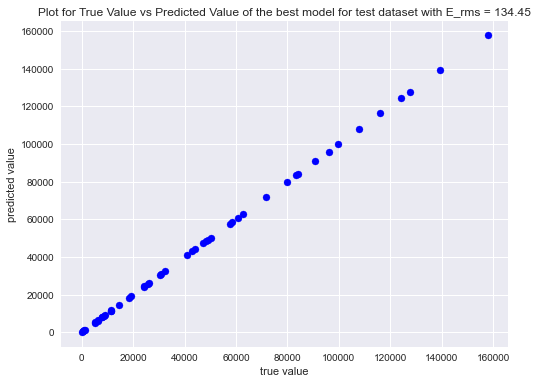
\includegraphics[height=1.6in]{Task3_new_images/batch500_test.png}
        \caption{Test Data }
    \end{subfigure}%
    \caption{Scatter Plot of the Gaussian Basis Function of the best performing model for Dataset 2}
    \label{fig:17}
\end{figure}

%%%%%%%%%%%%%%%%%%%%%%%%%%%%%%%%%%%%%%%%%%%%%%%%%%%%%%%%%%%%%%%%%%%%%%%%%%%%%%%%%%%%%%%%%%%%%%%%%%%%%%%%%%%%%%%%%%%%%%%%%%%%%%%%%%%%%%%%%%%%%%%%%%%%%%%%%%%%%%%%%%%%%%%%%%%%%%%%%%%%%%%%%%%%%%%%%%%%%%%%%%%%%%%%%%%%%%%%%%%%%%%%%%%%%%%%%%%%%%%%%%%%%%%%%%%%%%%%%%%%%%%%%%%%%%%%%%%%%%%%%%%%%%%%%%%%%


% \subsection{Experiments $\And$ Observations on Dataset 3:}

% \begin{figure}[!ht]
%     \centering
%         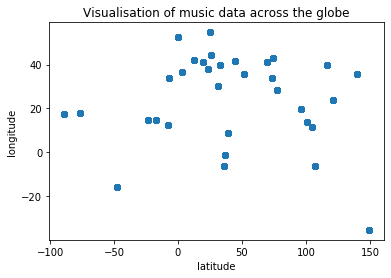
\includegraphics[height=3.2in]{Task 3 Images/Visualisation of music data across the globe.png}
%         \caption{Training Data}
% \end{figure}
\newpage
\section{Linear Model for Regression using Gaussian Basis Functions}
\subsection{\textcolor{teal}{Python Code}}

\begin{minted}[frame=lines, linenos, fontsize=\large]
{python}

# -*- coding: utf-8 -*-


import numpy as np
import pandas as pd
import matplotlib.pyplot as plt

################################ Dataset 3 ###################################

def process_dataset_3(D, var, r):
    
    """
    D: No of gauss functions for fit
    var: variance for fit
    r: regularisation term
    """
    # Read txt file
    
    f = open('datasets/2_music.txt', 'r')
    
    length = 0
    for line in f:
        
        d = [float(i) for i in line.split(',')]
        
        if length == 0:
            data = np.array(d)
            data = data[np.newaxis,:]
        else:
            d = np.array(d)
            d = d[np.newaxis,:]
            data = np.append(data,d,axis=0)
        length = length+1
    
    f.close()
       
    data = pd.DataFrame(data)
    
    
    # shuffle dataset
    data = data.sample(frac=1)
    
    # get dependent and independent varaible
    data = np.array(data)
    
    
    X = data[:,0:-2]
    y = data[:,-2:]
    
    # get unique values of y
    y_unique = np.unique(y,axis=0)
    
    # length of data for fit
    train_len = int(np.shape(X)[0]*0.7)
    val_len = int(np.shape(X)[0]*0.2)
    test_len = int(np.shape(X)[0]) - val_len - train_len
    
    # test train split
    X_train = X[0:train_len]
    X_test = X[train_len:train_len+test_len]
    X_val = X[train_len+test_len:train_len+test_len+val_len]
    
    y_train = y[0:train_len]
    y_test = y[train_len:train_len+test_len]
    y_val = y[train_len+test_len:train_len+test_len+val_len]
    
    # K-means clustering
    loop = 1
    prev_zni = np.zeros((train_len,D-1))
    
    while(loop>0):
        zni = np.zeros((train_len,D-1))
        
        if loop == 1:
            # randomly choose k points
            random_index = np.random.randint(0,train_len,D-1)
        
            # Initialize MUi
            MUi = X_train[random_index,:]
        
        # Determine points belonging to clusters
        for j in range(0,train_len):
            i = np.argmin(np.linalg.norm(X_train[j,:]-MUi,axis=1),axis=0)
            zni[j,i] = 1
            
        # Determine number of datapoints in the clusters
        Ni = np.sum(zni,axis=0)
        
        # Update MUi
        for j in range(0,D-1):
            if Ni[j] == 0:
                continue
            
            z = zni[:,j]
            MUi[j,:] = (np.sum(X_train*z[:,np.newaxis],axis=0))/Ni[j]
            
        # compare previous and current Zni
        comp = prev_zni - zni
        
        prev_zni = zni
        loop = loop+1
        
        # if no change break the loop
        if np.max(comp) == 0 and np.min(comp) == 0:
            break
    
    # Assign Mui
    mu = MUi
    
    # gaussian function
    phii = lambda x,mu : np.e**(-(np.linalg.norm(x-mu))/var**2)
    
    # Formulate phi matrix for training data
    phin = np.zeros((train_len,D))
    
    for i in range(0,train_len):
        for j in range(0,D):
            if j==0:
                phin[i,j] = 1
                #phin[i,j] = phii(X_train[i,:],mu[j,:])
            else:
                phin[i,j] = phii(X_train[i,:],mu[j,:])
            
    # weights with quadratic regularisation
    W = np.linalg.inv(phin.T@phin + r*np.identity(D))@phin.T@y_train
    
    # weights with tikhanov regularisation
    # phin_bar = np.zeros((D,D))
    # for i in range(0,D):
    #     for j in range(0,D):
    #         phin_bar[i,j] = np.exp(np.linalg.norm(mu[i,:]-mu[j,:])/var**2)
    
    # W = np.linalg.inv(phin.T@phin + r*phin_bar)@phin.T@y_train
    
    ###########################################################################
    
    # Test on training dataset
    y_pred = np.zeros((train_len,2))
    
    # Formulate phi matrix for training data
    phin = np.zeros((train_len,D))
    
    for i in range(0,train_len):
        for j in range(0,D):
            if j==0:
                phin[i,j] = 1
                # phin[i,j] = phii(X_train[i,:],mu[j,:])
            else:
                phin[i,j] = phii(X_train[i,:],mu[j])
    
    for i in range(0,train_len):
        pred = (phin[i,:])@W
        y_pred[i,:] = pred
        
        # term1 = np.deg2rad((pred[0] - y_unique[:,0])/2)
        # term2 = np.deg2rad((pred[1] - y_unique[:,1])/2)
        # a = (np.sin(term1)**2) + # np.cos(np.deg2rad(pred[0]))*
        #      np.cos(np.deg2rad(y_unique[:,0]))*(np.sin(term2# )**2)
        # dist = 2*6373*np.arctan2(np.sqrt(a),np.sqrt(1-a))
        
        # index = np.argmin(dist)
        # y_pred[i,:] = y_unique[index,:]
    
    Erms_train1 = ((np.linalg.norm(y_pred[:,0]-y_train[:,0])))/np.sqrt(train_len)
    Erms_train2 = ((np.linalg.norm(y_pred[:,1]-y_train[:,1])))/np.sqrt(train_len)

    # # scatter plot
    # fig1 = plt.figure(figsize=(9,9))
    # plt.scatter(y_train[:,0],y_pred[:,0],marker='x')
    # plt.scatter(y_train[:,1],y_pred[:,1],marker='x')
    # plt.xlabel('target',fontsize=20)
    # plt.ylabel('predicted',fontsize=20)
    # plt.title("Gaussian Basis Function (For Dataset 3 of # best performing 
    #             model with training data) | degree = {} | # lambda = {}".format(D,r),
    #             fontsize = 20)
    # plt.legend(["y0","y1"])
    ###########################################################################
    
    # Test on validation dataset
    y_pred = np.zeros((val_len,2))
    
    # Formulate phi matrix for validation data
    phin = np.zeros((val_len,D))
    
    for i in range(0,val_len):
        for j in range(0,D):
            if j==0:
                phin[i,j] = 1
                # phin[i,j] = phii(X_val[i,:],mu[j,:])
            else:
                phin[i,j] = phii(X_val[i,:],mu[j])
    
    for i in range(0,val_len):
        pred = (phin[i,:])@W
        y_pred[i,:] = pred
    
    
    Erms_val1 = ((np.linalg.norm(y_pred[:,0]-y_val[:,0])))/np.sqrt(val_len)
    Erms_val2 = ((np.linalg.norm(y_pred[:,1]-y_val[:,1])))/np.sqrt(val_len)
    
    # scatter plot for validation data
    # fig1 = plt.figure(figsize=(9,9))
    # plt.scatter(y_val,y_pred,marker='x')
    # plt.xlabel('target',fontsize=20)
    # plt.ylabel('predicted',fontsize=20)
    # plt.title("Gaussian Basis Function (For Dataset 2 of best performing model 
    #            with validation data) | degree = {} | lambda # = {}".format(D,r),
    #             fontsize = 20)
    
    ###############################################################################
    
    # Test on test dataset
    y_pred = np.zeros((test_len,2))
    
    # Formulate phi matrix for test data
    phin = np.zeros((test_len,D))
    
    for i in range(0,test_len):
        for j in range(0,D):
            if j==0:
                phin[i,j] = 1
                #phin[i,j] = phii(X_test[i,:],mu[j,:])
            else:
                phin[i,j] = phii(X_test[i,:],mu[j])
    
    for i in range(0,test_len):
        pred = (phin[i,:])@W
        y_pred[i,:] = pred
        
    Erms_test1 = ((np.linalg.norm(y_pred[:,0]-y_test[:,0])))/np.sqrt(test_len)
    Erms_test2 = ((np.linalg.norm(y_pred[:,1]-y_test[:,1])))/np.sqrt(test_len)
    
    # scatter plot for test data
    fig1 = plt.figure(figsize=(9,9))
    plt.scatter(y_test[:,0],y_pred[:,0],marker='x')
    plt.scatter(y_test[:,1],y_pred[:,1],marker='x')
    plt.xlabel('target',fontsize=20)
    plt.ylabel('predicted',fontsize=20)
    plt.title("Gaussian Basis Function (For Dataset 3 of best performing model
               with test data) | degree = {} | lambda = {}".format(D,r),
                fontsize = 20)
    plt.legend(["y0","y1"])
    ###########################################################################
    return Erms_train1, Erms_train2, Erms_val1, Erms_val2, Erms_test1, Erms_test2
    
################################ Dataset 2 ###################################

def process_dataset_2(D, var, r):
    
    """
    D: No of gauss functions for fit
    var: variance for fit
    r: regularisation term
    """
    
    # Read csv file
    data = pd.read_csv('datasets/function1_2d.csv')
    
    # shuffle dataset
    # data = data.sample(frac=1)
    
    # get dependent and independent varaible
    X = data[['x1','x2']]
    y = data['y']
    
    # convert into numpy
    X = np.array(X)
    y = np.array(y)
    
    # length of data for fit
    train_len = int(np.shape(X)[0]*0.7)
    test_len = int(np.shape(X)[0]*0.2)
    val_len = int(np.shape(X)[0]*0.1)
    
    # test train split
    X_train = X[0:train_len]
    X_test = X[train_len:train_len+test_len]
    X_val = X[train_len+test_len:train_len+test_len+val_len]
    
    y_train = y[0:train_len]
    y_test = y[train_len:train_len+test_len]
    y_val = y[train_len+test_len: train_len+test_len+val_len]
    
    # K-means clustering
    loop = 1
    prev_zni = np.zeros((train_len,D-1))
    
    while(loop>0):
        zni = np.zeros((train_len,D-1))
        
        if loop == 1:
            # randomly choose k points
            random_index = np.random.randint(0,train_len,D-1)
        
            # Initialize MUi
            MUi = X_train[random_index,:]
        
        # Determine points belonging to clusters
        for j in range(0,train_len):
            i = np.argmin(np.linalg.norm(X_train[j,:]-MUi,axis=1),axis=0)
            zni[j,i] = 1
            
        # Determine number of datapoints in the clusters
        Ni = np.sum(zni,axis=0)
        
        # Update MUi
        for j in range(0,D-1):
            if Ni[j] == 0:
                continue
            
            z = zni[:,j]
            MUi[j,:] = (np.sum(X_train*z[:,np.newaxis],axis=0))/Ni[j]
            
        # compare previous and current Zni
        comp = prev_zni - zni
        
        prev_zni = zni
        loop = loop+1
        
        # if no change break the loop
        if np.max(comp) == 0 and np.min(comp) == 0:
            break
    
    # Assign Mui
    mu = MUi
    
    # gaussian function
    phii = lambda x,mu : np.e**(-(np.linalg.norm(x-mu))/var**2)
    
    # Formulate phi matrix for training data
    phin = np.zeros((train_len,D))
    
    for i in range(0,train_len):
        for j in range(0,D):
            if j==0:
                phin[i,j] = 1
            else:
                phin[i,j] = phii(X_train[i,:],mu[j-1,:])
            
    
    # weights with quadratic regularisation
    W = np.linalg.inv(phin.T@phin + r*np.identity(D))@phin.T@y_train
    
    ###########################################################################
    
    # Test on training dataset
    y_pred = np.zeros((train_len,1))
    
    # Formulate phi matrix for training data
    phin = np.zeros((train_len,D))
    
    for i in range(0,train_len):
        for j in range(0,D):
            if j==0:
                phin[i,j] = 1
            else:
                phin[i,j] = phii(X_train[i,:],mu[j-1])
    
    for i in range(0,train_len):
        y_pred[i,:] = (phin[i,:])@W
        
    Erms_train = ((np.linalg.norm(y_pred-y_train[:,np.newaxis])))/
                   np.sqrt(train_len)
    
    
    # # scatter plot for training data
    # fig1 = plt.figure(figsize=(9,9))
    # plt.scatter(y_train,y_pred,marker='x')
    # plt.xlabel('target',fontsize=20)
    # plt.ylabel('predicted',fontsize=20)
    # plt.title("Gaussian Basis Function (For Dataset 2 of best performing model
    #             with training data) | degree = {} | lambda = # {}".format(D,r),
    #              fontsize = 20)
    
    
    ###########################################################################
    
    # Test on validation dataset
    y_pred = np.zeros((val_len,1))
    
    # Formulate phi matrix for validation data
    phin = np.zeros((val_len,D))
    
    for i in range(0,val_len):
        for j in range(0,D):
            if j==0:
                phin[i,j] = 1
            else:
                phin[i,j] = phii(X_val[i,:],mu[j-1])
    
    for i in range(0,val_len):
        y_pred[i,:] = (phin[i,:])@W
        
    Erms_val = ((np.linalg.norm(y_pred-y_val[:,np.newaxis])))/np.sqrt(val_len)
    
    # scatter plot for validation data
    # fig1 = plt.figure(figsize=(9,9))
    # plt.scatter(y_val,y_pred,marker='x')
    # plt.xlabel('target',fontsize=20)
    # plt.ylabel('predicted',fontsize=20)
    # plt.title("Gaussian Basis Function (For Dataset 2 of best performing model 
    #             with validation data) | degree = {} | lambda #= {}".format(D,r),
    #              fontsize = 20)
    
    ###########################################################################
    
    # Test on test dataset
    y_pred = np.zeros((test_len,1))
    
    # Formulate phi matrix for test data
    phin = np.zeros((test_len,D))
    
    for i in range(0,test_len):
        for j in range(0,D):
            if j==0:
                phin[i,j] = 1
            else:
                phin[i,j] = phii(X_test[i,:],mu[j-1])
    
    for i in range(0,test_len):
        y_pred[i,:] = (phin[i,:])@W
        
    Erms_test = ((np.linalg.norm(y_pred-y_test[:,np.newaxis])))/np.sqrt(test_len)
    
    # # scatter plot for validation data
    # fig1 = plt.figure(figsize=(9,9))
    # plt.scatter(y_test,y_pred,marker='x')
    # plt.xlabel('target',fontsize=20)
    # plt.ylabel('predicted',fontsize=20)
    # plt.title("Gaussian Basis Function (For Dataset 2 of best performing 
    #             model with test data) | degree = {} | lambda # = {}".format(D,r),
    #              fontsize = 20)
    
    ###########################################################################
    return Erms_train, Erms_val, Erms_test
    

############################ Main Code ########################################

# Call function to experiment dataset 2/3
D = [2,3,6,9,20,33,40,100]
var = [1,3,5,10,50,100]
reg = [0,10e-5,10e-4,10e-3,10e-2,10e-1,10,10e2,10e3,10e4,10e5]

Erms = []
# Experiment with variance
for v in var:
    erms = process_dataset_3(100, v, 0)
     Erms.append(erms)
    
# Plot table
fig = plt.figure(figsize=(9,9))
row_labels=["var = 1", "var = 3", "var = 5", "var = 10", "var = 50", "var = 100"]
column_labels=["Erms_train", "Erms_val", "Erms_test"]
column_labels=["Erms_train_y0","Erms_train_y1", "Erms_val0","Erms_val1",
                 "Erms_test0", "Erms_test1"]
plt.axis('tight')
plt.axis('off')
plt.table(cellText=Erms,rowLabels=row_labels,colLabels=column_labels, loc="center")

Erms = []
# Experiment with Dimensions
for d in D:
    erms = process_dataset_3(d, 3, 0)
    Erms.append(erms)

# Plot table
fig = plt.figure(figsize=(9,9))
row_labels=["D = 2", "D = 3", "D = 6", "D = 9", "D = 20", "D = 30",
              "D = 40", "D = 100"]
column_labels=["Erms_train", "Erms_val", "Erms_test"]
column_labels=["Erms_train_y0","Erms_train_y1", "Erms_val0","Erms_val1", 
                 "Erms_test0", "Erms_test1"]
plt.axis('tight')
plt.axis('off')
plt.table(cellText=Erms,rowLabels=row_labels,colLabels=column_labels,
            loc="center")

Erms = []  
# Experiment with regularisation
for r in reg:
    erms = process_dataset_3(100, 3, r)
    Erms.append(erms)
    
# Plot table
fig = plt.figure(figsize=(9,9))
row_labels=["lambda = 0", "lambda = 10e-5", "lambda = 10e-4", "lambda = 10e-3", 
              "lambda = 10e-2", "lambda = 10e-1", "lambda = 10", "lambda = 10e2", 
              "lambda = 10e3", "lambda = 10e4", "lambda = 10e5"]
column_labels=["Erms_train", "Erms_val", "Erms_test"]
column_labels=["Erms_train_y0","Erms_train_y1", "Erms_val0","Erms_val1", 
                 "Erms_test0", "Erms_test1"]
plt.axis('tight')
plt.axis('off')
plt.table(cellText=Erms,rowLabels=row_labels,colLabels=column_labels,
            loc="center")
\end{minted}

\newpage
% %\section*{List of Tables}
{\rowcolors{3}{green!40!yellow!10}{green!0!yellow!30}
\begin{table}[b]
\begin{tabular}{ |p{1.5cm}|p{3cm}|p{3cm}| p{3cm}|  }
\hline
\multicolumn{4}{|c|}{$\mathbf{E}_{rms}$ values for different data } \\
\hline
\rowcolor{lightgray} \textbf{Degree} & $\mathbf{E}_{rms-train}$ & $\mathbf{E}_{rms-test}$ & $\mathbf{E}_{rms-valid}$ \\
\hline
 3   &   0.9463088173826781  &  0.921529001681974   &  0.9948945706586969   \\   
 \hline
 6   &   0.09359023977652957   &   0.10083584398441547   &   0.09288903271612758         \\
 \hline
 9   &   0.09325227809164291   &    0.09456183788436022        &     0.10820363428341415     \\
 \hline
 15  &   0.09478479954779334    &     0.10579059792367092    &     0.10503728364765512     \\
 \hline
 20  &   0.09894796631401077  &    0.12511924445979059       &     0.11111596719234638      \\
 \hline
 40  &   273.11809897016593     &     280.49354546509295       &       264.14720043776646   \\
\hline
\end{tabular}
\caption{Error comparisons for varying degrees of $\phi(\mathbf{x}) $ for Dataset 1 using 50 samples}
\label{table:1}
\end{table}
}

{\rowcolors{3}{green!40!yellow!10}{green!0!yellow!30}
\begin{table}[b]
\begin{tabular}{ |p{1.5cm}|p{3cm}|p{3cm}| p{3cm}|  }
\hline
\multicolumn{4}{|c|}{$\mathbf{E}_{rms}$ values for different data } \\
\hline
\rowcolor{lightgray} $\lambda$ & $\mathbf{E}_{rms-train}$ & $\mathbf{E}_{rms-test}$ & $\mathbf{E}_{rms-valid}$ \\
\hline
 0.01  &  3.394572970966565     &       2.6317009238108264  &   3.147114587206947   \\   
 \hline
 0.1   &    0.10331454624525277   & 0.10897035717888424  & 0.12300118478086215         \\
 \hline
  1   &  0.17279386194186552   &     0.2035128106547716   &    0.13799626775817317   \\
 \hline
 10   &    0.6198124917211572   &     0.6066334675587216   &    0.725542005508596  \\
 \hline
 1000  &   3.229382540133771      &    3.3007384785428413     &     3.378847808304533      \\
\hline
\end{tabular}
\caption{Error comparisons for varying regularisation parameter for Dataset 1 using 50 samples}
\label{table:2}
\end{table}
}

\newpage

{\rowcolors{3}{green!40!yellow!10}{green!0!yellow!30}
\begin{table}[t]
\centering
\scalebox{0.80}{\begin{tabular}{ |p{1.0cm}|p{3.5cm}|p{3.5cm}| p{3.5cm}|  }
\hline
\multicolumn{4}{|c|}{$\mathbf{E}_{rms}$ values for different data } \\
\hline
\rowcolor{lightgray} \textbf{$\lambda$} & $\mathbf{E}_{rms-train}$ & $\mathbf{E}_{rms-test}$ & $\mathbf{E}_{rms-valid}$ \\
\hline
 1   &   7.580971664599636e-06  &  1.0605170215401277e-05   &  7.515845677117264e-06   \\   
 \hline
 0   &   12127947174797588e-07   &   1.156094643149333e-07  &   1.1747549893556596e-07         \\
 \hline
 0.1   &   7.755542491206345e-0   &    1.0655343968936e-06     &     7.77470171577322e-07     \\
 \hline
 0.01  &   1.0437989846157205e-07    &    1.316541941688553e-07   &     1.0167993899988677e-07    \\
 \hline
 0.001  &   1.1864030383147943e-07  &    1.0847674423224485-07       &     1.1773784421319634e-07      \\
 \hline
 0.0001  &   3.304880776430471e-08     &     3.229622737638675e-08      &      3.082385661556587e-08   \\
 \hline
 1e-05   &   1.776442992865663e-07    &     1.6570808617669024e-07      &     16951478603716152e-07  \\
\hline
\end{tabular}}
\caption{Error comparisons for varying values of $\lambda $ for Dataset 2 and a model of $degree = 6$}.
\label{table:3}
\end{table}
}

{\rowcolors{3}{green!40!yellow!10}{green!0!yellow!30}
\begin{table}[p]
\begin{tabular}{ |p{1.5cm}|p{3cm}|p{3cm}| p{3cm}|  }
\hline
\multicolumn{4}{|c|}{$\mathbf{E}_{rms}$ values for different data } \\
\hline
\rowcolor{lightgray} \textbf{$\lambda$} & $\mathbf{E}_{rms-train}$ & $\mathbf{E}_{rms-test}$ & $\mathbf{E}_{rms-valid}$ \\
\hline
 2   &   8472.094191227668  &  7916.242009164154  &  11603.319421097342   \\   
 \hline
 3   &   7746.879448478453   &   10209.228853144015  &   9055.030938196933     \\
 \hline
 6   &   1.1117446982463445e-06   &    7.120999286364823e-06     &     1.03246244720662512-06    \\
\hline
\end{tabular}
\caption{Error comparisons for varying degrees $\phi(\mathbf{x}) $ for Dataset 1 using 50 samples}.
\label{table:4}

 \vspace*{\floatsep}
 \begin{tabular}{ |p{1.5cm}|p{3cm}|p{3cm}| p{3cm}|  }
\hline
\multicolumn{4}{|c|}{$\mathbf{E}_{rms}$ values for different data } \\
\hline
\rowcolor{lightgray} \textbf{$\lambda$} & $\mathbf{E}_{rms-train}$ & $\mathbf{E}_{rms-test}$ & $\mathbf{E}_{rms-valid}$ \\
\hline
 2   &   7836.931386632586  &  9102.679593164155 &  10203.596869348119   \\   
 \hline
 3   &   7410.9365635257855   &   8955.316097382489  &   9615.301820662606     \\
 \hline
 6   &   9.077850586058267e-08   &    1.1420271837609817e-07     &     9.065940029841168e-08    \\
\hline
\end{tabular}
\caption{Error comparisons for varying degrees $\phi(\mathbf{x}) $ for Dataset 1 using 100 samples}.
\label{table:5}

\vspace*{\floatsep}
 \begin{tabular}{ |p{1.5cm}|p{3cm}|p{3cm}| p{3cm}|  }
\hline
\multicolumn{4}{|c|}{$\mathbf{E}_{rms}$ values for different data } \\
\hline
\rowcolor{lightgray} \textbf{$\lambda$} & $\mathbf{E}_{rms-train}$ & $\mathbf{E}_{rms-test}$ & $\mathbf{E}_{rms-valid}$ \\
\hline
 2   &   9007.857130881312  &  9941.501015342938 & 7712.903374733729   \\   
 \hline
 3   &   8891.048471356644   &   10448.970914479978  &   7669.043772436963    \\
 \hline
 6   &   2.7797471788073487e-08   &    3.158634266244641e-08     &     3.171659049297458e-08   \\
\hline
\end{tabular}
\caption{Error comparisons for varying degrees $\phi(\mathbf{x}) $ for Dataset 1 using 200 samples}.
\label{table:6}

\vspace*{\floatsep}
 \begin{tabular}{ |p{1.5cm}|p{3cm}|p{3cm}| p{3cm}|  }
\hline
\multicolumn{4}{|c|}{$\mathbf{E}_{rms}$ values for different data } \\
\hline
\rowcolor{lightgray} \textbf{$\lambda$} & $\mathbf{E}_{rms-train}$ & $\mathbf{E}_{rms-test}$ & $\mathbf{E}_{rms-valid}$ \\
\hline
 2   &   9308.742569191712  &  9968.552684122154 & 9908.81299031691   \\   
 \hline
 3   &   9237.93538859271   &   9721.986403575836  &   10117.449491662008    \\
 \hline
 6   &   2.541280516466242e-08   &    2.923416086330338e-08     &     2.515778040590836e-08  \\
\hline
\end{tabular}
\caption{Error comparisons for varying degrees $\phi(\mathbf{x}) $ for Dataset 1 using 500 samples}.
\label{table:7}
\end{table}
}

{\rowcolors{3}{green!40!yellow!10}{green!0!yellow!30}
\begin{table}[hptb]
\begin{tabular}{ |p{1.5cm}|p{3cm}|p{3cm}| p{3cm}|  }
\hline
\multicolumn{4}{|c|}{$\mathbf{E}_{rms}$ values for different data } \\
\hline
\rowcolor{lightgray} \textbf{Dimension} & $\mathbf{E}_{rms-train}$ & $\mathbf{E}_{rms-val}$ & $\mathbf{E}_{rms-test}$ \\
\hline
  2   &   20742.417961375482    &       19314.336433527136    &     20051.47268871791   \\
 \hline
 3   &   15755.436189348633    &       15039.506378963442    &     15602.040608854932   \\   
 \hline
 6   &   14465.019060036939    &       14170.647936247557    &     14146.981889693609         \\
 \hline
 9   &   9215.113706469303     &       9244.777763533128     &     8648.719452138206     \\
 \hline
 20  &   6043.52872279345      &       5996.571277859385     &     6128.169849741222     \\
 \hline
 30  &   4780.139930356894     &       4667.322597766088     &     4681.781287505215      \\
 \hline
 40  &   3250.5764084440207    &       3330.783324829522     &     3247.7191047865876     \\  
 \hline
 100 &   1454.005863919257     &       1609.951973441829     &     1580.1611713736224     \\
\hline
\end{tabular}
\caption{Error comparisons for varying dimensions of $\phi(\mathbf{x}) $ for Dataset 2}
\label{table:8}
\end{table}
}

{\rowcolors{3}{green!40!yellow!10}{green!0!yellow!30}
\begin{table}[hptb]
\begin{tabular}{ |p{1.5cm}|p{3cm}|p{3cm}| p{3cm}|  }
\hline
\multicolumn{4}{|c|}{$\mathbf{E}_{rms}$ values for different data } \\
\hline
\rowcolor{lightgray} \textbf{Variance} & $\mathbf{E}_{rms-train}$ & $\mathbf{E}_{rms-val}$ & $\mathbf{E}_{rms-test}$ \\
\hline
  1   &   27266.067337673085     &       26794.717392625018       &     20051.47268871791   \\
 \hline
  10   &   3656.998466228972     &       3735.493387300531        &     3906.388733286057   \\   
 \hline
  20  &  3955.814282945206       &       4130.987734108473        &     4077.2036579847054        \\
 \hline
  30  &   3448.199977857502      &       3590.5182818874255       &     3441.4907182960355     \\
 \hline
  50  &   3344.7152080262267     &       3317.3693879440525       &     3299.934482599632     \\
 \hline
  100  &   3460.736021173579     &       3586.197518340341        &     3471.484357305657      \\
\hline
\end{tabular}
\caption{Error comparisons for varying variance of $\phi(\mathbf{x}) $ for Dataset 2}
\label{table:9}
\end{table}
}


{\rowcolors{3}{green!40!yellow!10}{green!0!yellow!30}
\begin{table}[hptb]
\begin{tabular}{ |p{1.5cm}|p{3cm}|p{3cm}| p{3cm}|  }
\hline
\multicolumn{4}{|c|}{$\mathbf{E}_{rms}$ values for different data } \\
\hline
\rowcolor{lightgray}\textbf{$\lambda$} & $\mathbf{E}_{rms-train}$ & $\mathbf{E}_{rms-val}$ & $\mathbf{E}_{rms-test}$ \\
\hline
  0      &   1397.932974026646    &       1410.9028219564577       &     1545.4716845597673   \\
 \hline
  10e-5  &   3964.4172602252547    &       3870.2365010758563        &     3849.030700922454   \\   
 \hline
  10e-4  &  8711.736211556994       &       7773.878856448405        &     8852.914573070351        \\
 \hline
  10e-3  &   15352.219047826447      &       14113.981029840956       &     15308.868272544152     \\
 \hline
  10e-2  &   23555.54821056003      &       22613.32447875262       &     23171.93371145183    \\
 \hline
  10e-1  &   35560.49095521766     &       33790.609053408574        &     34783.161122408135      \\
  \hline
  10     &   38899.73825135093    &        36755.95627333107         &     38013.62049175868      \\
  \hline
  10e2   &   39374.00056336752    &         37152.40595020841       &      38408.5229340378        \\
  \hline
  10e3   &   39462.66115053631   &        37202.5849146428         &       38427.786409380235      \\
  \hline
  10e4   &   42522.79510032822   &         40234.01328931874       &        41188.57306560426      \\
  \hline
  10e5  &    51525.586833163274  &         49441.16118608065       &        50036.24559820878      \\
\hline
\end{tabular}
\caption{Error comparisons for varying regularisation parameter of quadratic regularisation for Dataset 2}
\label{table:10}
\end{table}
}

{\rowcolors{3}{green!40!yellow!10}{green!0!yellow!30}
\begin{table}[tb]
\scalebox{0.55}{\begin{tabular}{ |p{1.5cm}|p{3cm}|p{3cm}| p{3cm}| p{3cm}|p{3cm}| p{3cm}|  }
\hline
\multicolumn{7}{|c|}{$\mathbf{E}_{rms}$ values for different data } \\
\hline
\rowcolor{lightgray} Dimension & $\mathbf{E}_{rms-train-y0}$ & $\mathbf{E}_{rms-train-y1}$ & $\mathbf{E}_{rms-val0}$ & $\mathbf{E}_{rms-val1}$ &  $\mathbf{E}_{rms-test0}$ &  $\mathbf{E}_{rms-test1}$ \\
\hline
  2     &   18.261846789547043    &       50.65695100540773       &     19.840639029197767       &   51.06873345746765  &    18.254833582438298  &  48.95919177851435 \\
 \hline
  3     &   17.334954893345568    &       48.12017274970571        &     18.706214741786283      &    49.71352945145123  &    17.17314618212547  &   47.724961836340945 \\   
 \hline
  6     &  17.21724620357916       &       46.99705049021136       &     18.834661130384912      &    49.634431632314964  &    17.163879951147674  &  45.94363248661904 \\
 \hline
  9     &   17.077105017870227      &       46.87369239679521       &     18.77092894123055      &     49.87652992771683   &    17.052167362078986  &   46.10645522423818\\
 \hline
  20    &   16.62495158941184     &       44.061507191733746       &     18.93496242535791        &     47.45628326015504  &     17.23914191898175   &   44.92890562234594\\
 \hline
  33  &   16.012300063409644    &       41.79895682697146        &     18.075549490984013         &      46.78349566044533  &     17.097226654252182  &   43.57425350042887\\
  \hline
  40     &   15.030462151159838    &        41.44975397428952         &     16.19277786217412     &      46.69485632012707  &      16.65992841822436  &    44.81158342803822    \\
  \hline
  100   &   13.55811902615394    &         36.907588168775035       &      15.80489133721302     &        44.12021164076166  &     16.015682127814014  &    43.131276345243805   \\
\hline
\end{tabular}}
\caption{Error comparisons for varying dimensions of $\phi(\mathbf{x}) $ for Dataset 3}
\label{table:11}
\end{table}
}


{\rowcolors{3}{green!40!yellow!10}{green!0!yellow!30}
\begin{table}[hptb]
\scalebox{0.55}{\begin{tabular}{ |p{1.5cm}|p{3cm}|p{3cm}| p{3cm}| p{3cm}|p{3cm}| p{3cm}|  }
\hline
\multicolumn{7}{|c|}{$\mathbf{E}_{rms}$ values for different data } \\
\hline
\rowcolor{lightgray} Variance & $\mathbf{E}_{rms-train-y0}$ & $\mathbf{E}_{rms-train-y1}$ & $\mathbf{E}_{rms-val0}$ & $\mathbf{E}_{rms-val1}$ &  $\mathbf{E}_{rms-test0}$ &  $\mathbf{E}_{rms-test1}$ \\
\hline
  1     &   14.802082001368419   &       40.321633889977555       &     18.674698016763532       &   49.129937352270495  &    17.531128868461472  &  46.76344308207428 \\
 \hline
  3     &   13.346329858456485    &       36.62961663677716        &     15.764064151476793      &    45.81525148776968  &    16.520541317683545  &   46.76344308207428 \\   
 \hline
  5     &  13.640579634337296       &       36.186648455886434       &     15.812790126872471      &    44.63374844449026  &    16.511763175509085  &  43.67856796701367 \\
 \hline
  10     &   14.0987218470415      &       36.778109183602       &     16.26421539249013      &     46.88670651092855   &    16.405458185345264  &   43.156236717132145\\
 \hline
  50    &   13.674845030840684     &       36.29889121262914       &     15.781700370044856        &     45.74320900614563  &     16.731671336916644   &   45.5138057637192\\
 \hline
  100  &   13.782864959175388    &       36.01806523216255        &     15.294067216827727         &      45.4569107646632  &     16.753307582782714  &   45.39844353123662\\
\hline
\end{tabular}}
\caption{Error comparisons for varying variance of $\phi(\mathbf{x}) $ for Dataset 3}
\label{table:12}
\end{table}
}

{\rowcolors{3}{green!40!yellow!10}{green!0!yellow!30}
\begin{table}[tb]
\scalebox{0.55}{\begin{tabular}{ |p{1.5cm}|p{3cm}|p{3cm}| p{3cm}| p{3cm}|p{3cm}| p{3cm}|  }
\hline
\multicolumn{7}{|c|}{$\mathbf{E}_{rms}$ values for different data } \\
\hline
\rowcolor{lightgray} $\lambda$ & $\mathbf{E}_{rms-train-y0}$ & $\mathbf{E}_{rms-train-y1}$ & $\mathbf{E}_{rms-val0}$ & $\mathbf{E}_{rms-val1}$ &  $\mathbf{E}_{rms-test0}$ &  $\mathbf{E}_{rms-test1}$ \\
\hline
  0     &   13.66088377149326   &       37.285766888657555      &     15.927056611439305       &   44.69227818303191  &    16.661375141900336  &  43.648244255376284 \\
 \hline
  10e-5     &   13.773461052064862   &       37.03424408415342        &     16.066732976968748      &   43.62865894352013  &    16.242967641419053  &   43.36750441328951 \\   
 \hline
  10e-4     &  13.766829901791684       &       37.3578462638808       &     15.785850683393287      &    44.63889473802704  &    16.610303825911128  &  43.3866754847842 \\
 \hline
  10e-3     &   13.668866314769637     &       37.03966259762649      &     16.41969987078999     &     45.21998805255312   &    16.32697303255949  &   43.463508314498505\\
 \hline
  10e-2    &   13.925275904633729     &       38.257785271001346       &     16.58147942231442        &     45.636260077067696  &     16.378607987589707  &   43.063921790118336\\
 \hline
  10e-1  &   15.534821033284558   &       41.81525227305627        &     17.800568817319125    &      46.65333516922764  &     16.721016020353698  &  43.945624996788695\\
 \hline
  10     &   16.9176516020855   &   46.486079296414204       &    19.01222579708267   &     47.98663870405902   &  17.157649876534602  &  45.898772862385975   \\
 \hline
  10e2   &   19.159237169328758       &   52.19830606619423   &    20.95977882810739     &     50.947437218140095   &   18.87822713135429  &  49.21334507326434  \\
 \hline 
 10e3    &    24.332577966987376        &   56.72759899039606    &  25.917646274832467    &    54.85790377017556    &    23.41251511304732  &  52.472092842546495 \\
 \hline
 10e4    &    31.05307877592449     &     63.05254607021164      &   32.38823488158862 &   60.90692188787098      &     29.992995680479932  &  58.35106811530104 \\
 \hline  
 10e5    &    32.334369135654136    &        64.34034977054226       &   33.63128917230101  &   62.1597016014964   &     31.267653630611612  &   59.59797143564928 \\
\hline
\end{tabular}}
\caption{Error comparisons for varying regularisation parameter of quadratic regularisation for Dataset 3}
\label{table:13}
\end{table}
}



{\rowcolors{3}{green!40!yellow!10}{green!0!yellow!30}
\begin{table}[h]
\scalebox{0.55}{\begin{tabular}{ |p{1.5cm}|p{3cm}|p{3cm}| p{3cm}| p{3cm}|p{3cm}| p{3cm}|  }
\hline
\multicolumn{7}{|c|}{$\mathbf{E}_{rms}$ values for different data } \\
\hline
\rowcolor{lightgray} $\lambda$ & $\mathbf{E}_{rms-train-y0}$ & $\mathbf{E}_{rms-train-y1}$ & $\mathbf{E}_{rms-val0}$ & $\mathbf{E}_{rms-val1}$ &  $\mathbf{E}_{rms-test0}$ &  $\mathbf{E}_{rms-test1}$ \\
\hline
  0     &   13.890754554969238   &       37.41730553208801       &     16.11287838871868       &   44.51861811577798  &    16.534599199117768  &  43.9288716513483 \\
 \hline
  10e-5     &   14.485719956192346   &       38.39484490501671        &     17.2763227095301      &   46.430843265365716  &    16.68197571099453  &   43.24925713306916 \\   
 \hline
  10e-4     &  13.767912927166181       &       36.641001158338256       &     15.936124599084282      &    45.829561599290024  &    16.692571285468837  &  43.68620454521084 \\
 \hline
  10e-3     &   13.513817115754222      &       36.84397379341463       &     15.58930066852842      &     45.30494111423051   &    17.16690499566545  &   43.729591351277534\\
 \hline
  10e-2    &   108.12639556208411     &       386.9273742160467       &     65.10234547482186        &     240.35522218899126  &     65.02440846657572  &   265.2471344902372\\
 \hline
  10e-1  &   63.82946354737652   &       143.12517039925356        &     48.52563721901755    &      106.07277405310934  &     43.617860204005304  &  103.7567712344792\\
 \hline
  10     &   25.127576488517068    &   70.03489629315638        &    26.224425890196866   &     63.53212554938365   &   25.42797143222253   &  62.41227564233563   \\
 \hline
  10e2   &   32.40392998142076       &   64.5359123363723    &    34.019020127236004     &      62.27211488636792   &   31.464248629812158  &  59.89563753309275  \\
 \hline 
 10e3    &    32.6468064341186        &   64.64944787570482    &  33.94995764268507     &     62.478490736654486    &    31.581504727322397  &  59.900747817710695 \\
 \hline
 10e4    &    32.506353586950446     &     64.51533413201933      &   33.799603360247396  &   62.3316116230041      &     31.439573655316625  &  59.76808091578914 \\
 \hline  
 10e5    &    32.49211458098274    &         64.5012420864329       &   33.78454195623247  &   62.316636220168476   &     31.4247182620759   &   59.75411611922825  \\
\hline
\end{tabular}}
\caption{Error comparisons for varying regularisation parameter of Tikhonov regularisation for Dataset 3}
\label{table:14}
\end{table}
}







% \newpage
% %\section*{List of Figures}
\begin{figure}[b]
    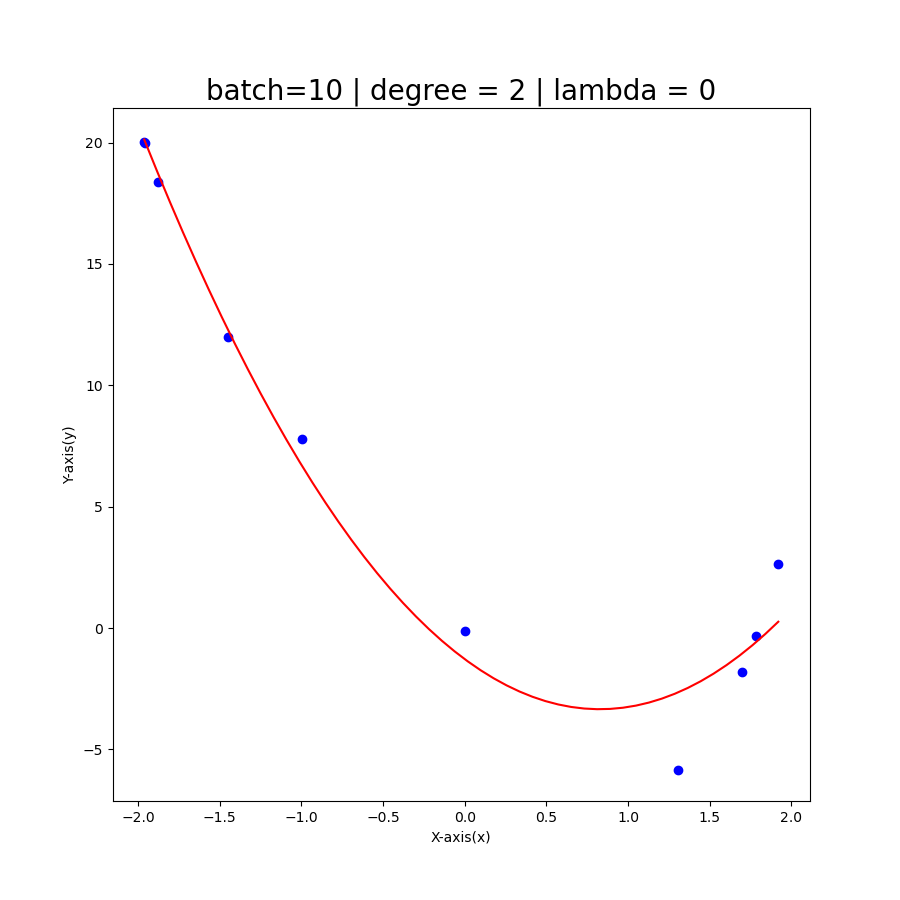
\includegraphics[width=.24\textwidth]{Task 1 Images/Batch 10/Figure_1.png}\hfill
    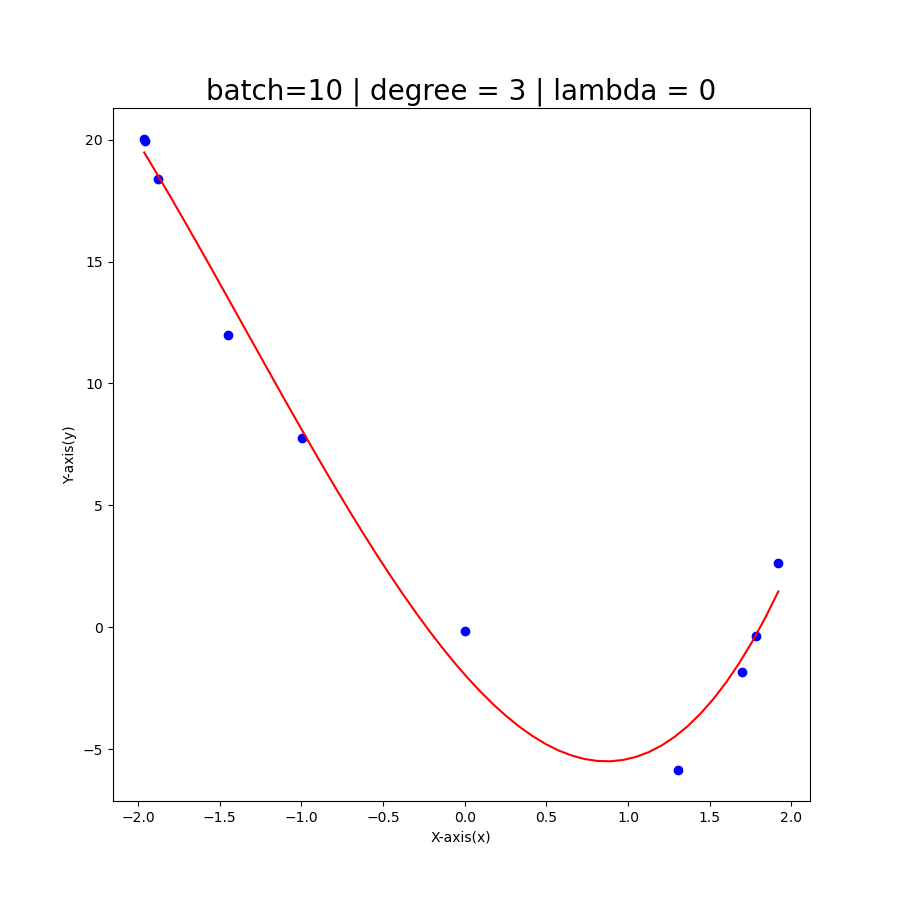
\includegraphics[width=.24\textwidth]{Task 1 Images/Batch 10/Figure_2.png}\hfill
    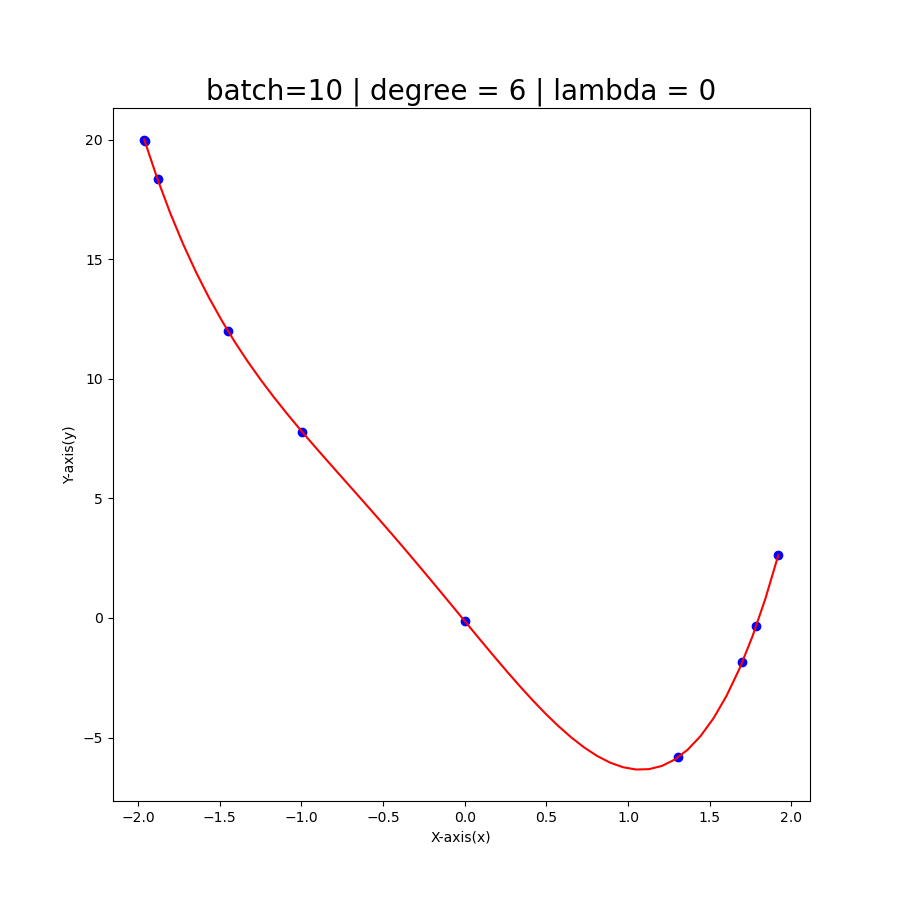
\includegraphics[width=.24\textwidth]{Task 1 Images/Batch 10/Figure_3.png}\hfill
    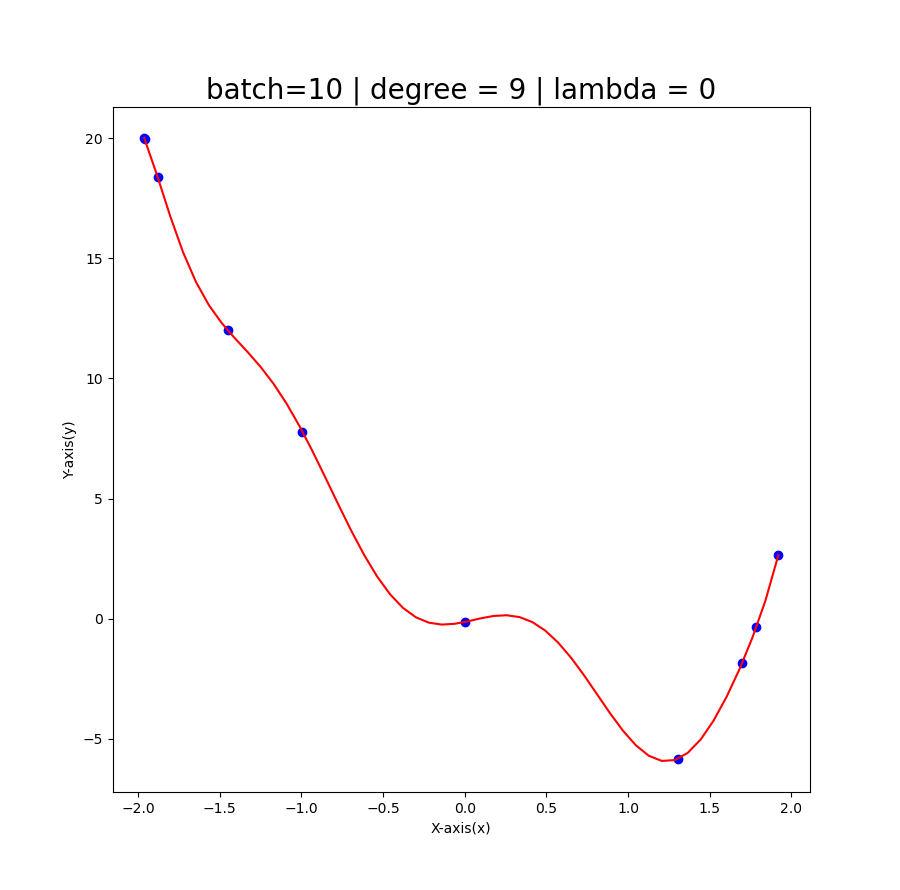
\includegraphics[width=.24\textwidth]{Task 1 Images/Batch 10/Figure_4.png}
    \caption{Plots of Polynomials having various orders of degree for a fixed regularistion parameter $\lambda = 0$ using 10 samples}
    \label{fig:1}
    \vspace*{\floatsep}

    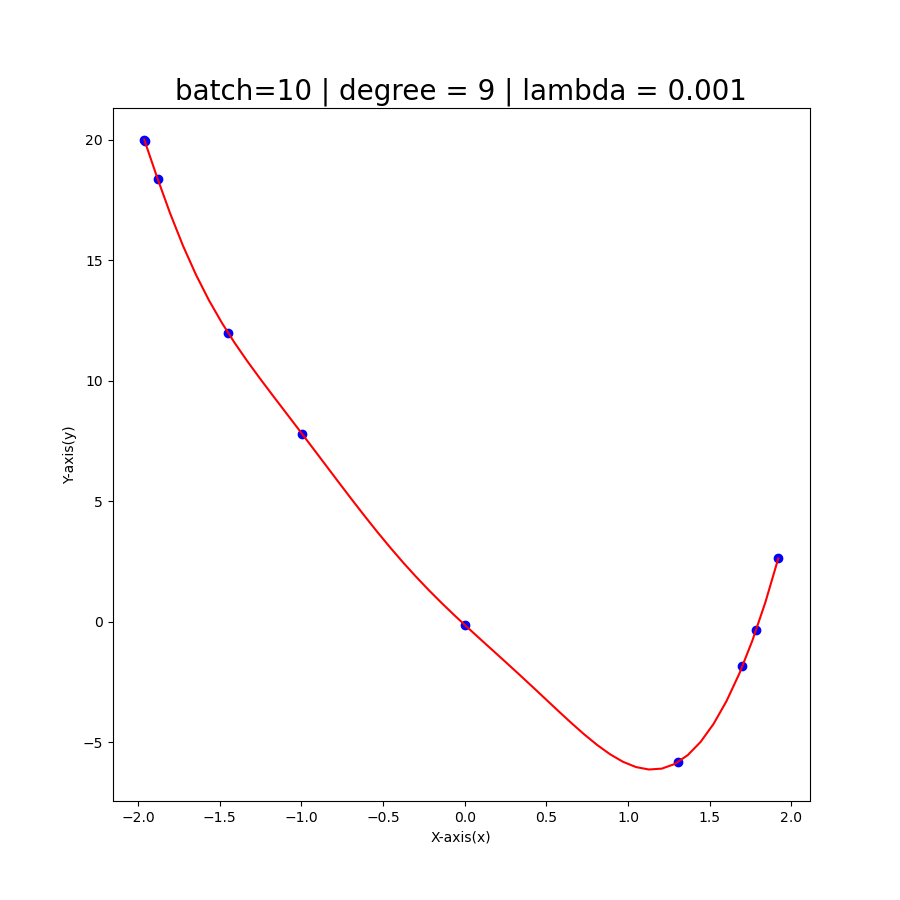
\includegraphics[width=.24\textwidth]{Task 1 Images/Batch 10/Figure_5.png}\hfill
    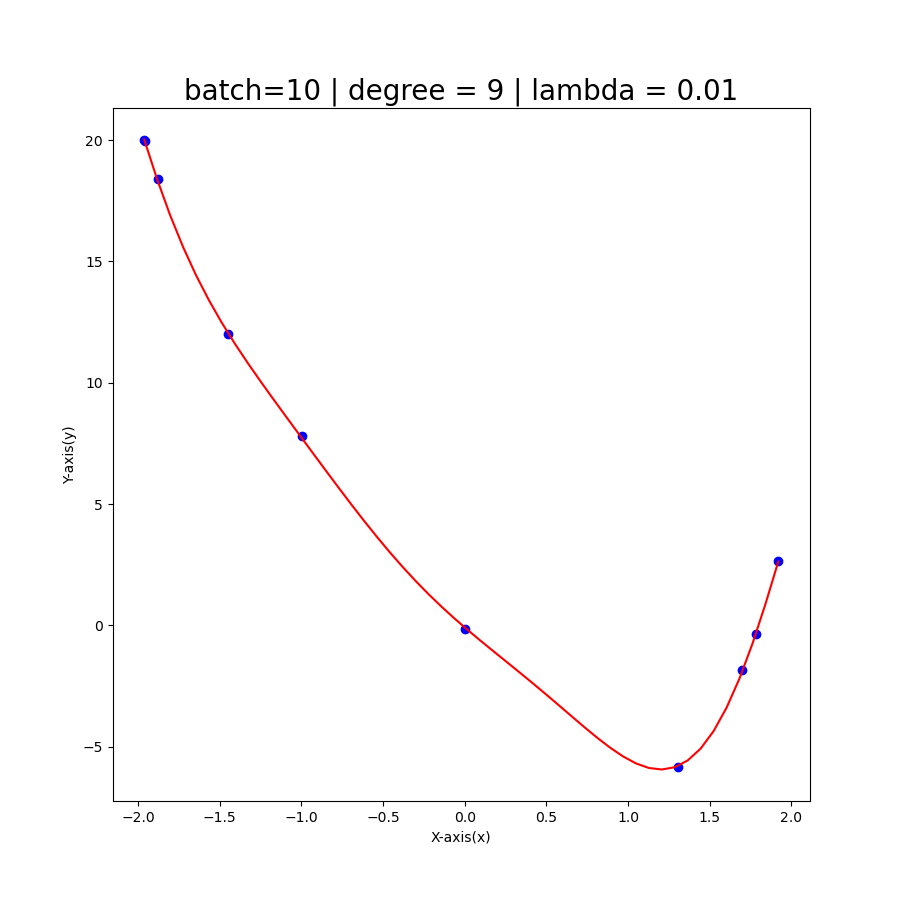
\includegraphics[width=.24\textwidth]{Task 1 Images/Batch 10/Figure_6.png}\hfill
    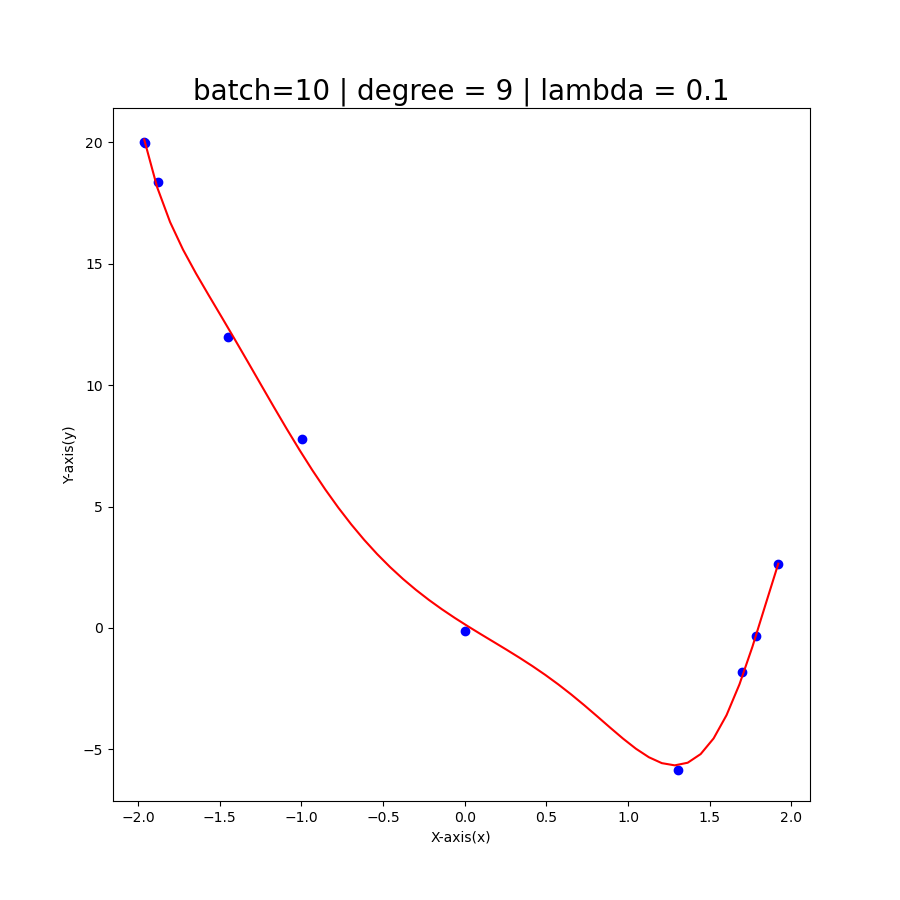
\includegraphics[width=.24\textwidth]{Task 1 Images/Batch 10/Figure_7.png}\hfill
    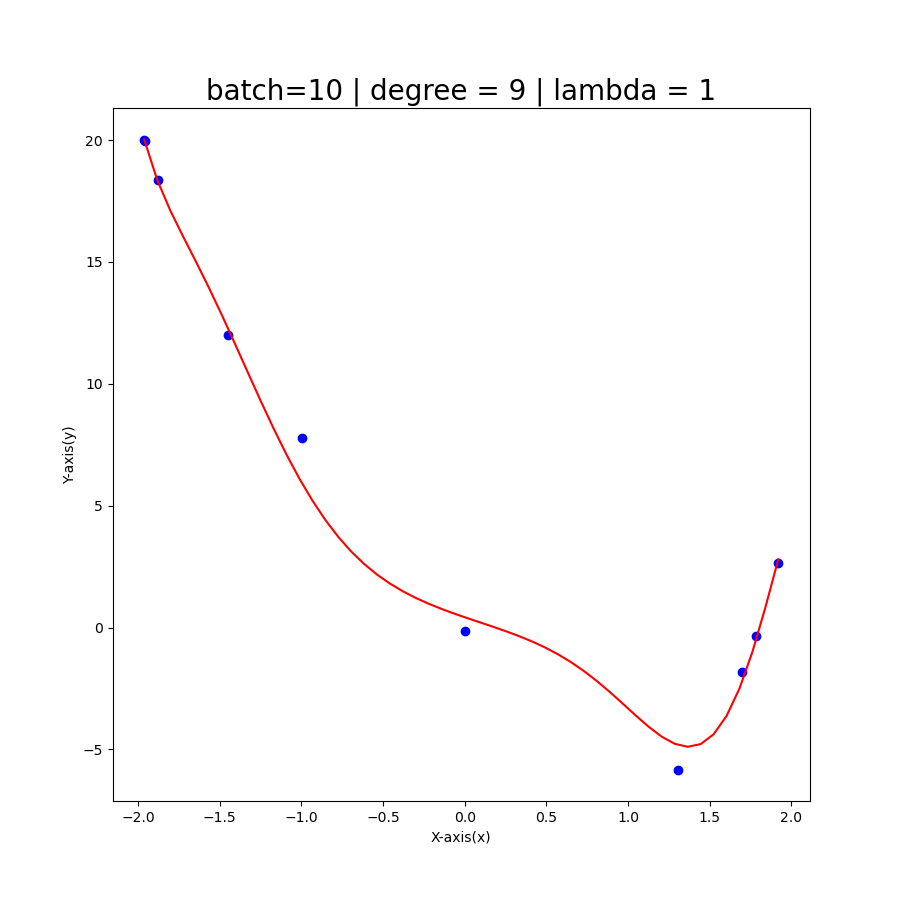
\includegraphics[width=.24\textwidth]{Task 1 Images/Batch 10/Figure_8.png}
    \caption{Plots of Polynomials having various orders of degree for a fixed regularisation parameter $\lambda = 1$ using 10 samples}
    \label{fig:2}
    \vspace*{\floatsep}

    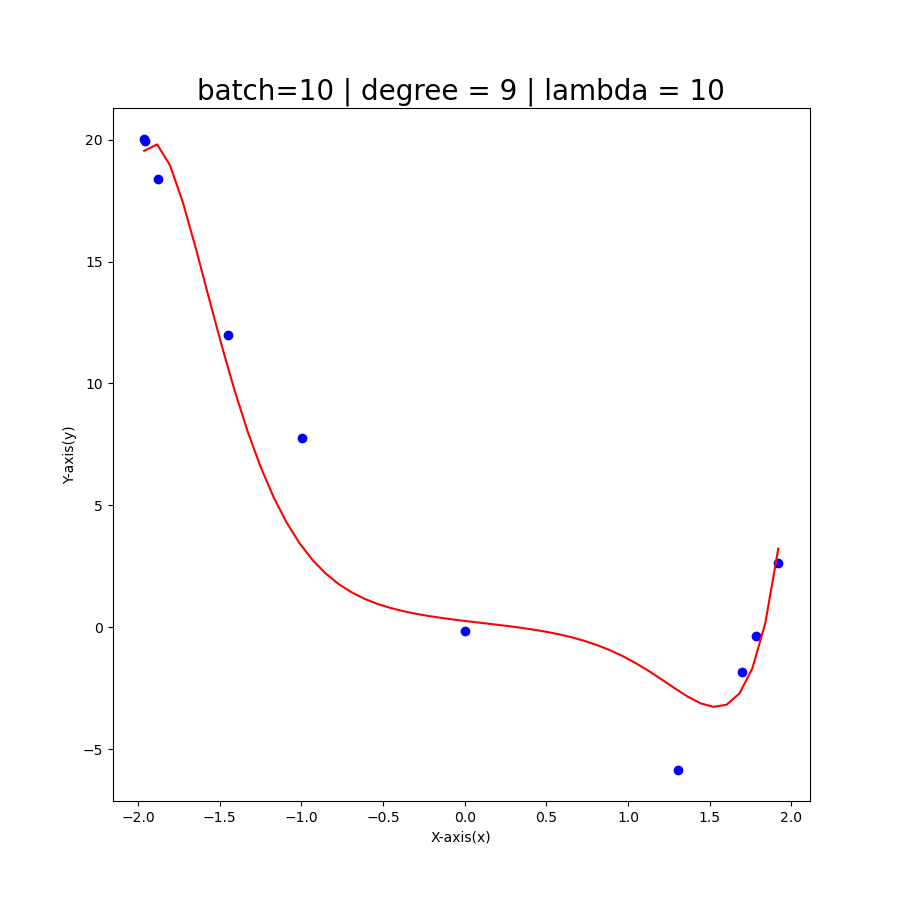
\includegraphics[width=.24\textwidth]{Task 1 Images/Batch 10/Figure_9.png}\hfill
    \includegraphics[width=.24\textwidth]{Task 1 Images/Batch 10/Figure_10.png}\hfill
    \includegraphics[width=.24\textwidth]{Task 1 Images/Batch 10/Figure_11.png}\hfill
    \includegraphics[width=.24\textwidth]{Task 1 Images/Batch 10/Figure_12.png}
    \caption{Plots of Polynomials having various orders of degree for a fixed regularisation parameter $\lambda = 0.1$ using 10 samples}
    \label{fig:3}
    \vspace*{\floatsep}

    \includegraphics[width=.24\textwidth]{Task 1 Images/Batch 10/Figure_13.png}\hfill
    \includegraphics[width=.24\textwidth]{Task 1 Images/Batch 10/Figure_14.png}\hfill
    \includegraphics[width=.24\textwidth]{Task 1 Images/Batch 10/Figure_15.png}\hfill
    \includegraphics[width=.24\textwidth]{Task 1 Images/Batch 10/Figure_16.png}
    \caption{Plots of Polynomials having various orders of degree for a fixed regularisation parameter $\lambda = 10$ using 10 samples}
    \label{fig:4}
\end{figure}    
    %\vspace*{\floatsep}
\begin{figure}[p]
    \includegraphics[width=.24\textwidth]{Task 1 Images/Batch 10/Figure 17.png}\hfill
    \includegraphics[width=.24\textwidth]{Task 1 Images/Batch 10/Figure 18.png}\hfill
    \includegraphics[width=.24\textwidth]{Task 1 Images/Batch 10/Figure 19.png}\hfill
    \includegraphics[width=.24\textwidth]{Task 1 Images/Batch 10/Figure 20.png}
    \caption{Plots of Polynomials having various orders of degree for a fixed regularisation parameter $\lambda = 1000$ using 10 samples}
    \label{fig:5}
    \vspace*{\floatsep}
    
    \includegraphics[width=.24\textwidth]{Task 1 Images/Batch 50/Figure 1.png}\hfill
    \includegraphics[width=.24\textwidth]{Task 1 Images/Batch 50/Figure 2.png}\hfill
    \includegraphics[width=.24\textwidth]{Task 1 Images/Batch 50/Figure 3.png}\hfill
    \includegraphics[width=.24\textwidth]{Task 1 Images/Batch 50/Figure 4.png}
    \caption{Plots of Polynomials having various orders of degree for a fixed regularisation parameter $\lambda = 0$ using 50 samples}
    \label{fig:6}
    \vspace*{\floatsep}
    
    \includegraphics[width=.24\textwidth]{Task 1 Images/Batch 50/Figure 5.png}\hfill
    \includegraphics[width=.24\textwidth]{Task 1 Images/Batch 50/Figure 6.png}\hfill
    \includegraphics[width=.24\textwidth]{Task 1 Images/Batch 50/Figure 7.png}\hfill
    \includegraphics[width=.24\textwidth]{Task 1 Images/Batch 50/Figure 8.png}
    \caption{Plots of Polynomials having various orders of degree for a fixed regularisation parameter $\lambda = 1$ using 50 samples}
    \label{fig:7}
    \vspace*{\floatsep}
    
    \includegraphics[width=.24\textwidth]{Task 1 Images/Batch 50/Figure 9.png}\hfill
    \includegraphics[width=.24\textwidth]{Task 1 Images/Batch 50/Figure 10.png}\hfill
    \includegraphics[width=.24\textwidth]{Task 1 Images/Batch 50/Figure 11.png}\hfill
    \includegraphics[width=.24\textwidth]{Task 1 Images/Batch 50/Figure 12.png}
    \caption{Plots of Polynomials having various orders of degree for a fixed regularisation parameter $\lambda = 0.1$ using 50 samples}
    \label{fig:8}
\end{figure}

\begin{figure}[p]
   \includegraphics[width=.24\textwidth]{Task 1 Images/Batch 50/Figure 13.png}\hfill
    \includegraphics[width=.24\textwidth]{Task 1 Images/Batch 50/Figure 14.png}\hfill
    \includegraphics[width=.24\textwidth]{Task 1 Images/Batch 50/Figure 15.png}\hfill
    \includegraphics[width=.24\textwidth]{Task 1 Images/Batch 50/Figure 16.png}
    \caption{Plots of Polynomials having various orders of degree for a fixed regularisation parameter $\lambda = 10$ using 50 samples}
    \label{fig:9}
    \vspace*{\floatsep}

    \includegraphics[width=.24\textwidth]{Task 1 Images/Batch 50/Figure 17.png}\hfill
    \includegraphics[width=.24\textwidth]{Task 1 Images/Batch 50/Figure 18.png}\hfill
    \includegraphics[width=.24\textwidth]{Task 1 Images/Batch 50/Figure 19.png}\hfill
    \includegraphics[width=.24\textwidth]{Task 1 Images/Batch 50/Figure_20.png}
    \caption{Plots of Polynomials having various orders of degree for a fixed regularisation parameter $\lambda = 1000$ using 50 samples}
    \label{fig:10}
    \vspace*{\floatsep}
\end{figure}
\newpage
\begin{figure}[b]
    \centering
    \begin{subfigure}[t]{0.25\textwidth}
        \centering
        \includegraphics[height=1in]{Task 2 Images/batch500_deg2_lambda.png}
        \caption{Degree, $M = 2$}
    \end{subfigure}%
    ~ 
    \begin{subfigure}[t]{0.25\textwidth}
        \centering
        \includegraphics[height=1in]{Task 2 Images/batch500_deg3_lambda.png}
        \caption{Degree, $M = 3$ }
    \end{subfigure}%
    ~
    \begin{subfigure}[t]{0.25\textwidth}
        \centering
        \includegraphics[height=1in]{Task 2 Images/batch500_deg6_lambda1to100.png}
        \caption{ Degree, $M = 6$}
    \end{subfigure}
    \caption{Effect of $\lambda$}
    \label{fig:11}
\end{figure}

\begin{figure}[p]
    \includegraphics[width=.30\textwidth]{Task 2 Images/surfaceplot_batch50_deg2_lamb0.png}\hfill
    \includegraphics[width=.30\textwidth]{Task 2 Images/surfaceplot_batch50_deg3_lamb0.png}\hfill
    \includegraphics[width=.30\textwidth]{Task 2 Images/surfaceplot_batch50_deg6_lamb0.png}
    \caption{Surface Plots using various degree for a fixed best regularisation parameter $\lambda = 0$ using 50 samples }
    \label{fig:12}
    \vspace*{\floatsep}
    
    \includegraphics[width=.30\textwidth]{Task 2 Images/surfaceplot_batch100_deg2_lamb0.png}\hfill
    \includegraphics[width=.30\textwidth]{Task 2 Images/surfaceplot_batch100_deg3_lamb0.png}\hfill
    \includegraphics[width=.30\textwidth]{Task 2 Images/surfaceplot_batch100_deg6_lamb0.png}
    \caption{Surface Plots using various degree for a fixed regularisation parameter $\lambda = 0$ using 100 samples}
    \label{fig:13}
    \vspace*{\floatsep}
    
    \includegraphics[width=.30\textwidth]{Task 2 Images/surfaceplot_batch200_deg2_lamb0.png}\hfill
    \includegraphics[width=.30\textwidth]{Task 2 Images/surfaceplot_batch200_deg2_lamb0.png}\hfill
    \includegraphics[width=.30\textwidth]{Task 2 Images/surfaceplot_batch200_deg2_lamb0.png}
    \caption{Surface Plots using various degree for a fixed regularisation parameter $\lambda = 0$ using 200 samples}
    \label{fig:14}
    \vspace*{\floatsep}
    
    \includegraphics[width=.30\textwidth]{Task 2 Images/surfaceplot_batch500_deg2_lamb0.png}\hfill
    \includegraphics[width=.30\textwidth]{Task 2 Images/surfaceplot_batch500_deg3_lamb0.png}\hfill
    \includegraphics[width=.30\textwidth]{Task 2 Images/surfaceplot_batch500_deg6_lamb0.png}
    \caption{Surface Plots using various degree for a fixed regularisation parameter $\lambda = 0$ using 500 samples}
    \label{fig:15}
\end{figure}

\begin{figure}[tb]
     \centering
     \begin{subfigure}[t]{0.30\textwidth}
         \centering
         \includegraphics[height=1.6in]{Task 2 Images/best_scatterplot_batch_500_degree_6_lambda_0_training.png}
         \caption{Training Data}
     \end{subfigure}%
     ~ 
     \begin{subfigure}[t]{0.30\textwidth}
         \centering
         \includegraphics[height=1.6in]{Task 2 Images/best_scatterplot_batch_500_degree_6_lambda_0_test.png}
         \caption{Test Data }
     \end{subfigure}%
     ~
     \begin{subfigure}[t]{0.30\textwidth}
         \centering
         \includegraphics[height=1.6in]{Task 2 Images/best_scatterplot_batch_500_degree_6_lambda_0_validation.png}
         \caption{Validation Data }
     \end{subfigure}
     \caption{Best Scatter Plot}
     \label{fig:16}
\end{figure}
\newpage
\begin{figure}[t]
    \centering
    \begin{subfigure}[t]{0.50\textwidth}
        \centering
        \includegraphics[height=1.6in]{Task 3 Images/3.1.42.png}
        \caption{Training Data}
    \end{subfigure}%
    ~ 
    \begin{subfigure}[t]{0.50\textwidth}
        \centering
        \includegraphics[height=1.6in]{Task 3 Images/3.1.41.png}
        \caption{Test Data }
    \end{subfigure}%
    \caption{Scatter Plot of the Gaussian Basis Function of the best performing model for Dataset 2}
    \label{fig:17}
\end{figure}

\begin{figure}[tb]
    \centering
    \begin{subfigure}[t]{0.50\textwidth}
        \centering
        \includegraphics[height=1.6in]{Task 3 Images/3.2.51.png}
        \caption{Training Data}
    \end{subfigure}%
    ~ 
    \begin{subfigure}[t]{0.50\textwidth}
        \centering
        \includegraphics[height=1.6in]{Task 3 Images/3.2.52.png}
        \caption{Test Data }
    \end{subfigure}%
    \caption{Scatter Plot of the Gaussian Basis Function of the best performing model for Dataset 3}
    \label{fig:18}
\end{figure}

%\bibliographystyle{unsrt}
\bibliography{ref}

% ------------------------------------------------------------------------------
% End document
% ------------------------------------------------------------------------------
\end{document}